%---------------------------------------------------------------------------%
%-                                                                         -%
%-                           LaTeX Template                                -%
%-                                                                         -%
%---------------------------------------------------------------------------%
%- Copyright (C) Huangrui Mo <huangrui.mo@gmail.com> 
%- This is free software: you can redistribute it and/or modify it
%- under the terms of the GNU General Public License as published by
%- the Free Software Foundation, either version 3 of the License, or
%- (at your option) any later version.
%---------------------------------------------------------------------------%
%->> Document class declaration
%---------------------------------------------------------------------------%
\documentclass[doublesided%,fontset=%adobe%fandol
,12pt]{Style/ucasthesis}%
%- Multiple optional arguments:
%- [<singlesided|doublesided|printcopy>]% set one or two sided eprint or print
%- [showmj]% show confidential information
%- [draftversion]% show draft version information
%- [fontset=<fandol|...>]% specify font set to replace automatic detection
%- [scheme=plain]% thesis writing of international students
%- [standard options for ctex book class: draft|paper size|font size|...]%
%---------------------------------------------------------------------------%
%->> Document settings
%---------------------------------------------------------------------------%
\usepackage[super,myhdr,list]{Style/artratex}% document settings
%- usage: \usepackage[option1,option2,...,optionN]{artratex}
%- Multiple optional arguments:
%- [bibtex|biber]% set bibliography processor and package
%- [<numbers|super|authoryear|alpha>]% set citation and reference style
%- <numbers>: textual: Jones [1]; parenthetical: [1]
%- <super>: textual: Jones superscript [1]; parenthetical: superscript [1]
%- <authoryear>: textual: Jones (1995); parenthetical: (Jones, 1995)
%- <alpha>: textual: not available; parenthetical: [Jon95]
%- [geometry]% reconfigure page layout via geometry package
%- [lscape]% provide landscape layout environment
%- [myhdr]% enable header and footer via fancyhdr package
%- [color]% provide color support via xcolor package
%- [background]% enable page background
%- [tikz]% provide complex diagrams via tikz package
%- [table]% provide complex tables via ctable package
%- [list]% provide enhanced list environments for algorithm and coding
%- [math]% enable some extra math packages
\usepackage{Style/artracom}% user defined commands
\usepackage{appendix}
\usepackage{pdfpages}
\usepackage{setspace}
\usepackage{enumerate}
\usepackage{enumitem}
\usepackage{amsthm}
\usepackage{amsmath}
%\usepackage{bicaption} % package for binary captions
%\captionsetup[figure][bi-second]{name=Figure} % the second figure caption name
%\captionsetup[table][bi-second]{name=Table} % the second table caption name
\renewcommand{\theequation}{\arabic{chapter}-\arabic{equation}}
\renewcommand{\thefigure}{\arabic{chapter}-\arabic{figure}}
\renewcommand{\thetable}{\arabic{chapter}-\arabic{table}}
\renewcommand{\contentsname}{目录\vspace{2cm}}
\renewcommand{\thesection}{\arabic{section}}
\renewcommand{\theequation}{ A.\arabic{equation}}%设置附录中公式显示样式
\setcounter{tocdepth}{3}           %增加目录深度
\setcounter{secnumdepth}{3}        %增加编号深度
       
%---------------%此处代码为修改目录层次显示不合适问题--------      
\makeatletter
\renewcommand*\l@section{\@dottedtocline{2}{1.8em}{1.2em}}
\renewcommand*\l@subsection{\@dottedtocline{3}{3.2em}{1.2em}}
\renewcommand*\l@subsubsection{\@dottedtocline{4}{5.2em}{1.2em}}
\makeatother
%--------------------数学环境——————————————————————————————————————————-
\newtheorem{theorem}{\hspace{2em}定理} [section]
\newtheorem{axiom}{\hspace{2em}公理} [section]
\newtheorem{lemma}{\hspace{2em}引理}[section]
\newtheorem{corollary}[]{\hspace{2em}推论}[section]
\newtheorem{assertion}{\hspace{2em}断言}[section]
\newtheorem{proposition}{\hspace{2em}命题} [section]
%\newtheorem{proof}{\hspace{2em}证明} 
\newtheorem{definition}{\hspace{2em}定义}
\newtheorem{example}{\hspace{2em}例子} [section]
\newtheorem{remark}{\hspace{2em}注}[section]
%-
%-----------------------设置默认字体和行距----------------
\usepackage{xeCJK}   %中文字体
\setCJKfamilyfont{kaitibold}{Kaiti SC Bold}
\newcommand{\kaitiB}{\CJKfamily{kaitibold}}   %楷体加粗
\setCJKfamilyfont{heitibold}{Source Han Sans CN}
\newcommand{\heitiB}{\CJKfamily{heitibold}}   %黑体加粗
\setCJKfamilyfont{songtibold}{Songti SC}
\newcommand{\songtiB}{\CJKfamily{songtibold}}   %宋体加粗
 \zihao{-4}\linespread{1.067}\selectfont
 %-------------------设置字体大小--------------
 %   命令  	大小(bp)     	意义
 %\zihao{0} 	42      	初号
 %\zihao{-0}	36          小初
 % \zihao{1}	26        	一号
 % \zihao{-1}	24      	小一
 % \zihao{2}	22      	二号
 % \zihao{-2}	18      	小二
 % \zihao{3}	16	        三号
 % \zihao{-3}	15	        小三
 % \zihao{4}	14      	四号
 % \zihao{-4}	12      	小四
 % \zihao{5}	10.5      	五号
 % \zihao{-5}	9         	小五
 % \zihao{6}	7.5	        六号
 % \zihao{-6}	6.5	        小六
 % \zihao{7}	5.5     	七号
 % \zihao{8}	5   	    八号
 


%---------------------------------------------------------------------------%
%------------定义页面大小----------------
%\usepackage{geometry}\geometry{	a4paper,	total={170mm,257mm},	left=20mm,	top=20mm,}
%->> Document inclusion
%---------------------------------------------------------------------------%
%\includeonly{Tex/Chap_1,...,Tex/Chap_N}% selected files compilation
%---------------------------------------------------------------------------%
%->> Document content
%---------------------------------------------------------------------------%
\begin{document}
%-
%-> Frontmatter: title page, abstract, content list, symbol list, preface
%-
\frontmatter% initialize the environment
%---------------------------------------------------------------------------%
%->> Titlepage information
%---------------------------------------------------------------------------%
%-
%\includepdfmerge{[pdfname],[a-b]}//pdfname 是pdf的名字,放当前目录下,a-b是引用的页数。
%
%\includepdfmerge{lwfmmm.pdf,1}
\includepdfmerge{fengmian.pdf,1-2}
%-> Chinese titlepage
%-
\confidential{}% confidential level
\schoollogo{scale=0.95}{wzu}% university logo
%\title{在光学腔中自旋压缩态产生的研究}% 
\title[温州大学硕士学位论文\LaTeX{}模板]{温州大学学位论文\LaTeX{}模板}
\author{刘刚}% name of author
\advisor{王明锋}% supervisor
\advisorsec{}% co-supervisor
\degree{硕士}% degree
\degreetype{理学}% degree type
\major{凝聚态物理}% major
\institute{温州大学}% institute of author
\chinesedate{2014~年~6~月}% customized date, 6 for summer and 12 for winter graduation
%-
%-> English titlepage
%-
\englishtitle{\LaTeX{} Thesis Template\\ of \\ WenZhou University}
\englishauthor{Huangrui Mo}
\englishadvisor{Supervisor: Professor Qingquan Liu}
\englishdegree{Master of Natural Science}% degree type <Doctor|Master> of <Philosophy|Natural Science|Engineering>
\englishthesistype{thesis}% thesis type <thesis|dissertation>
\englishmajor{Fluid Mechanics}% major
\englishinstitute{Institute of Mechanics, Chinese Academy of Sciences}
\englishdate{June, 2014}% customized date
%-
%-> Create titlepages
%-
%\maketitle
%\makeenglishtitle
%-
%-> Author's declaration
%-
\makedeclaration
%-
%-> Chinese abstract
%-

\chapter[摘要]{温州大学学位论文\LaTeX{}模板}
\vbox{}

\section*{\qquad\qquad\qquad\qquad\qquad\qquad\quad\  摘\quad 要}
\vbox{}
%\chaptermark{摘\quad 要}

\setcounter{page}{1}% set page number
\pagenumbering{Roman}% set large roman

{
	\par
	\zihao{4}
	\linespread{1.5}\selectfont
	
	
	本文是温州大学硕士学位论文模板,根据中国科学院大学学位论文模板ucasthesis修改而来,并依据其实用说明写了这份使用说明文档。主要内容为介绍\LaTeX{}文档类ucasthesis的用法,以及如何使用\LaTeX{}快速高效地撰写学位论文。
	
	
\par

\vbox{}
\keywords{温州大学,学位论文,\LaTeX{}模板}% 中文关键词
%-
%-> English abstract
%-

\chapter[Abstract]{\linespread{1.5}\selectfont \LaTeX{} Thesis Template of WenZhou University}

\vbox{}
\section*{\qquad\qquad\qquad\qquad\qquad\quad\quad ABSTRACT}
\vbox{}
%\chaptermark{Abstract}
%\vskip 1cm


{
	\par
	\zihao{4}
	\linespread{1.5}\selectfont
	
This paper is a help documentation for the \LaTeX{} class ucasthesis, which is  a thesis template for the University of WenZhou, which come from a thesis template for the University of Chinese Academy of Sciences. The main content is about how to use the ucasthesis, as well as how to write thesis efficiently by using \LaTeX{}.
	
	\par

\vbox{}
%\vskip 1cm
\englishkeywords{\linespread{1.5}\selectfont WenZhou University, Thesis, \LaTeX{} Template}% 英文关键词
%---------------------------------------------------------------------------%
% 摘要在这里修改
{% content list region
\linespread{1.2}% local line space
%
\tableofcontents% 显示目录
%\intotoc{\listfigurename}% 这里决定论文中是否显示图片索引
%\listoffigures% figures catalog
%\intotoc{\listtablename}% 这里决定论文中是否显示图表索引
%\listoftables% tables catalog
}
%\chapter*{符号列表}
\chaptermark{符号列表}

\section*{字符}
\nomenclatureitem[\textbf{Unit}]{\textbf{Symbol}}{\textbf{Description}}
\nomenclatureitem[$\Unit{m^{2} \cdot s^{-2} \cdot K^{-1}}$]{$R$}{the gas constant}
\nomenclatureitem[$\Unit{m^{2} \cdot s^{-2} \cdot K^{-1}}$]{$C_v$}{specific heat capacity at constant volume}
\nomenclatureitem[$\Unit{m^{2} \cdot s^{-2} \cdot K^{-1}}$]{$C_p$}{specific heat capacity at constant pressure}
\nomenclatureitem[$\Unit{m^{2} \cdot s^{-2}}$]{$E$}{specific total energy}
\nomenclatureitem[$\Unit{m^{2} \cdot s^{-2}}$]{$e$}{specific internal energy}
\nomenclatureitem[$\Unit{m^{2} \cdot s^{-2}}$]{$h_T$}{specific total enthalpy}
\nomenclatureitem[$\Unit{m^{2} \cdot s^{-2}}$]{$h$}{specific enthalpy}
\nomenclatureitem[$\Unit{kg \cdot m \cdot s^{-3} \cdot K^{-1}}$]{$k$}{thermal conductivity}
\nomenclatureitem[$\Unit{kg \cdot m^{-1} \cdot s^{-2}}$]{$S_{ij}$}{deviatoric stress tensor}
\nomenclatureitem[$\Unit{kg \cdot m^{-1} \cdot s^{-2}}$]{$\tau_{ij}$}{viscous stress tensor}
\nomenclatureitem[$\Unit{1}$]{$\delta_{ij}$}{Kronecker tensor}
\nomenclatureitem[$\Unit{1}$]{$I_{ij}$}{identity tensor}

\section*{算子}
\nomenclatureitem{\textbf{Symbol}}{\textbf{Description}}
\nomenclatureitem{$\Delta$}{difference}
\nomenclatureitem{$\nabla$}{gradient operator}
\nomenclatureitem{$\delta^{\pm}$}{upwind-biased interpolation scheme}

\section*{缩写}
\nomenclatureitem{CFD}{Computational Fluid Dynamics}
\nomenclatureitem{CFL}{Courant-Friedrichs-Lewy}
\nomenclatureitem{EOS}{Equation of State}
\nomenclatureitem{JWL}{Jones-Wilkins-Lee}
\nomenclatureitem{WENO}{Weighted Essentially Non-oscillatory}
\nomenclatureitem{ZND}{Zel'dovich-von Neumann-Doering}

% 这里决定论文中是否显示符号列表,对应文件可添加符号
%-
%-> Mainmatter
%-
\mainmatter% initialize the environment
%---------------------------------------------------------------------------%
%->> Main content
%---------------------------------------------------------------------------%
\chapter{引言}\label{chap:introduction}
\vbox{}\vbox{}
\section{研究背景}

考虑到许多同学可能缺乏\LaTeX{}使用经验,ucasthesis将\LaTeX{}的复杂性高度封装,开放出简单的接口,以便轻易使用。同时,对用\LaTeX{}撰写论文的一些主要难题,如制图、制表、文献索引等,进行了详细说明,并提供了相应的代码样本,理解了上述问题后,对于初学者而言,使用此模板撰写学位论文将不存在实质性的困难。所以,如果你是初学者,请不要直接放弃,因为同样为初学者的我,十分明白让\LaTeX{}简单易用的重要性,而这正是ucasthesis所追求和体现的。

此温州大学硕士学位论文\LaTeX{}模板是从中国科学院大学学位论文模板ucasthesis修改而来的,在修改过程中参考了温大硕士学位论文Word模板,虽然在修改过程中力图做到和word所要求格式一模一样,但鉴于本人水平有限且原Word模板中有部分效果不是特别美观,因此在最终输出效果上有一定的出入,请斟酌选择。此模板兼顾操作系统:Windows,Linux,MacOS 和\LaTeX{}编译引擎:pdflatex,xelatex,lualatex。支持中文书签、中文渲染、中文粗体显示、拷贝PDF中的文本到其他文本编辑器等特性。此外,对模板的文档结构进行了精心设计,撰写了编译脚本提高模板的易用性和使用效率。

本模板的目标在于简化学位论文的撰写,利用\LaTeX{}格式与内容分离的特征,模板将格式设计好后,作者可只需关注论文内容。 同时,本模板有着整洁一致的代码结构和扼要的注解,对文档的仔细阅读可为初学者提供一个学习\LaTeX{}的窗口。此外,模板的架构十分注重通用性,通过少量修改即可成为使用\LaTeX{}撰写中英文文章或书籍的通用模板,并为使用者的个性化设定提供了接口。

此模板非官方指定模板,请自行选择是否使用!

\section{系统要求}\label{sec:system}

\href{https://github.com/mohuangrui/ucasthesis}{\textbf{本模板}} 宏包可以在目前主流的 \href{https://en.wikibooks.org/wiki/LaTeX/Introduction}{\LaTeX{}} 编译系统中使用,如\TeX{}Live和MiK\TeX{}。因C\TeX{}套装已停止维护,\textbf{不再建议使用} (请勿混淆C\TeX{}套装与ctex宏包。C\TeX{}套装是集成了许多\LaTeX{}组件的\LaTeX{}编译系统。 \href{https://ctan.org/pkg/ctex?lang=en}{ctex} 宏包如同ucasthesis,是\LaTeX{}命令集,其维护状态活跃,并被主流的\LaTeX{}编译系统默认集成,是几乎所有\LaTeX{}中文文档的核心架构)。推荐的 \href{https://en.wikibooks.org/wiki/LaTeX/Installation}{\LaTeX{}编译系统} 和 \href{https://en.wikibooks.org/wiki/LaTeX/Installation}{\LaTeX{}文本编辑器} 为
\begin{center}
    %\footnotesize% fontsize
    %\setlength{\tabcolsep}{4pt}% column separation
    %\renewcommand{\arraystretch}{1.5}% row space 
    \begin{tabular}{lcc}
        \hline
        %\multicolumn{num_of_cols_to_merge}{alignment}{contents} \\
        %\cline{i-j}% partial hline from column i to column j
        操作系统 & \LaTeX{}编译系统 & \LaTeX{}文本编辑器\\
        \hline
        Linux & \href{https://www.tug.org/texlive/acquire-netinstall.html}{\TeX{}Live Full} & \href{http://www.xm1math.net/texmaker/}{Texmaker} 或 Vim \\
        MacOS & \href{https://www.tug.org/mactex/}{Mac\TeX{} Full} & \href{http://www.xm1math.net/texmaker/}{Texmaker} 或 Texshop\\
        Windows & \href{https://www.tug.org/texlive/acquire-netinstall.html}{\TeX{}Live Full} 或 \href{https://miktex.org/download}{MiK\TeX{}} & \href{http://www.xm1math.net/texmaker/}{Texmaker}\\
        \hline
    \end{tabular}
\end{center}

\LaTeX{}编译系统,如\TeX{}Live(Mac\TeX{}为针对MacOS的\TeX{}Live),用于提供编译环境,\LaTeX{}文本编辑器 (如Texmaker) 用于编辑\TeX{}源文件。请从各软件官网下载安装程序,勿使用不明程序源。\textbf{\LaTeX{}编译系统和\LaTeX{}编辑器分别安装成功后,即完成了\LaTeX{}的系统配置},无需其他手动干预和配置。若系统原带有旧版的\LaTeX{}编译系统并想安装新版,请\textbf{先卸载干净旧版再安装新版}。

\section{问题反馈}

关于\LaTeX{}的知识性问题,请查阅 \href{https://github.com/mohuangrui/ucasthesis/wiki}{ucasthesis知识小站} 和 \href{https://en.wikibooks.org/wiki/LaTeX}{\LaTeX{} Wikibook}。

关于模板编译和样式设计的问题,请\textbf{先仔细阅读此说明文档,特别是“常见问题”(章节~\ref{sec:qa})}。若问题仍无法得到解决,请\textbf{先将问题理解清楚并描述清楚,再将问题反馈}至 \href{https://github.com/mohuangrui/ucasthesis/issues}{Github/ucasthesis/issues}。

欢迎大家有效地反馈模板不足之处,一起不断改进模板。希望大家向同事积极推广\LaTeX{},一起更高效地做科研。

\section{模板下载}

\begin{center}
    \href{https://github.com/mohuangrui/ucasthesis}{Github/ucasthesis}: \url{https://github.com/mohuangrui/ucasthesis}
\end{center}

\chapter{\LaTeX{}使用说明}\label{chap:guide}
\vbox{}\vbox{}
为方便使用及更好地展示\LaTeX{}排版的优秀特性,该模板的框架和文件体系进行了细致地处理,尽可能地对各个功能和板块进行了模块化和封装,对于初学者来说,众多的文件目录也许一开始让人觉得有些无所适从,但阅读完下面的使用说明后,会发现原来使用思路是简单而清晰的,而且,当对\LaTeX{}有一定的认识和了解后,会发现其相对Word类排版系统极具吸引力的优秀特性。所以,如果是初学者,请不要退缩,请稍加尝试和坚持,以领略到\LaTeX{}的非凡魅力,并可以通过阅读相关资料如\LaTeX{} Wikibook \citep{wikibook2014latex} 来完善自己的使用知识。

\section{先试试效果}

\begin{itemize}
    \item 安装软件:根据所用操作系统和章节~\ref{sec:system}中的信息安装\LaTeX{}编译环境。
    \item 获取模板:下载 \href{https://github.com/mohuangrui/ucasthesis}{ucasthesis} 模板并解压。ucasthesis模板不仅提供了相应的类文件,同时也提供了包括参考文献等在内的完成学位论文的一切要素,所以,下载时,推荐下载整个ucasthesis文件夹,而不是单独的文档类。
    \item 编译模板:
        \begin{itemize}
            \item Windows:双击运行artratex.bat脚本。
            \item Linux或MacOS: {\scriptsize \verb|terminal| -> \verb|chmod +x ./artratex.sh| -> \verb|./artratex.sh xa|}
            \item 任意系统:都可使用\LaTeX{}编辑器打开Thesis.tex文件并选择xelatex编译引擎进行编译。
        \end{itemize}
    \item 错误处理:若编译中遇到了问题,请先查看“常见问题”(章节~\ref{sec:qa})。
\end{itemize}

编译完成即可获得本PDF说明文档。而这也完成了学习使用ucasthesis撰写论文的一半进程。什么?这就学成一半了,这么简单???,是的,就这么简单!

\section{文档目录简介}

\subsection{Thesis.tex}

Thesis.tex为主文档,其设计和规划了论文的整体框架,通过对其的阅读可以了解整个论文框架的搭建。

\subsection{编译脚本}

\begin{itemize}
	\item Windows:双击Dos脚本artratex.bat可得全编译后的PDF文档,其存在是为了帮助不了解\LaTeX{}编译过程的初学者跨过编译这第一道坎,请勿通过邮件传播和接收此脚本,以防范Dos脚本的潜在风险。
	\item Linux或MacOS:在terminal中运行
	\begin{itemize}
		\item \verb|./artratex.sh xa|:获得全编译后的PDF文档
		\item \verb|./artratex.sh x|:快速编译模式
	\end{itemize}
	\item 全编译指运行 \verb|xelatex+bibtex+xelatex+xelatex| 以正确生成所有的引用链接,如目录,参考文献及引用等。在写作过程中若无添加新的引用,则可用快速编译,即只运行一遍\LaTeX{}编译引擎以减少编译时间。
\end{itemize}

\subsection{Tmp文件夹}

运行编译脚本后,编译所生成的文档皆存于Tmp文件夹内,包括编译得到的PDF文档,其存在是为了保持工作空间的整洁,因为好的心情是很重要的。

\subsection{Style文件夹}

包含ucasthesis文档类的定义文件和配置文件,通过对它们的修改可以实现特定的模版设定。若需更新模板,一般只需用新的样式文件替换旧的即可。

\begin{itemize}
	\item ucasthesis.cls:文档类定义文件,论文的最核心的格式即通过它来定义的。
	\item ucasthesis.cfg:文档类配置文件,设定如目录显示为“目~录”而非“目录”。
	\item artratex.sty: 常用宏包及文档设定,如参考文献样式、文献引用样式、页眉页脚设定等。这些功能具有开关选项,常只需在Thesis.tex中的如下命令中进行启用即可,一般无需修改artratex.sty本身。
	
	\path{\usepackage[options]{artratex}} 
	\item artracom.sty:自定义命令以及添加宏包的推荐放置位置。
\end{itemize}

\subsection{Tex文件夹}

文件夹内为论文的所有实体内容,正常情况下,这也是\textbf{使用ucasthesis撰写学文论文时,主要关注和修改的一个位置,注:所有文件都必须采用UTF-8编码,否则编译后将出现乱码文本},详细分类介绍如下:

\begin{itemize}
	\item Frontpage.tex:为论文中英文封面及中英文摘要。\textbf{论文封面会根据英文学位名称如Bachelor,Master,或是Doctor自动切换为相应的格式}。
	\item Mainmatter.tex:索引需要出现的Chapter。开始写论文时,可以只索引当前章节,以快速编译查看,当论文完成后,再对所有章节进行索引即可。
	\item Chap{\_}xxx.tex:为论文主体的各个章节,可根据需要添加和撰写。
	\item Appendix.tex:为附录内容
	\item Backmatter.tex:为发表文章信息和致谢部分等。
\end{itemize}

\subsection{Img文件夹}

用于放置论文中所需要的图类文件,支持格式有:.jpg, .png, .pdf。其中,\verb|ucas_logo.pdf|为国科大校徽。不建议为各章节图片建子目录,即使图片众多,若命名规则合理,图片查询亦是十分方便。

\subsection{Biblio文件夹}

\begin{itemize}
	\item ref.bib:参考文献信息库。
	\item gbt7714-xxx.bst:文献样式定义文件。由 \href{https://github.com/zepinglee}{zepinglee}  开发,在最新国标的基础上对ucas进行了定制。与文献样式有关的问题,请查阅开发者所提供的文档,并建议适当追踪 \href{https://github.com/CTeX-org/gbt7714-bibtex-style/tree/ucas}{ucas 样式分支}的更新。
\end{itemize}


\section{数学公式、图表、参考文献等功能}

\subsection{数学公式}

比如Navier-Stokes方程(方程~\eqref{eq:ns}):
\begin{equation} \label{eq:ns}
%\adddotsbeforeeqnnum%
\begin{cases}
\frac{\partial \rho}{\partial t} + \nabla\cdot(\rho\Vector{V}) = 0 \ \mathrm{times\ math\ test: 1,2,3,4,5}, 1,2,3,4,5\\
\frac{\partial (\rho\Vector{V})}{\partial t} + \nabla\cdot(\rho\Vector{V}\Vector{V}) = \nabla\cdot\Tensor{\sigma} \ \text{times text test: 1,2,3,4,5}\\
\frac{\partial (\rho E)}{\partial t} + \nabla\cdot(\rho E\Vector{V}) = \nabla\cdot(k\nabla T) + \nabla\cdot(\Tensor{\sigma}\cdot\Vector{V})
\end{cases}
\end{equation}
\begin{equation}
%\adddotsbeforeeqnnum%
\frac{\partial }{\partial t}\int\limits_{\Omega} u \, \mathrm{d}\Omega + \int\limits_{S} \unitVector{n}\cdot(u\Vector{V}) \, \mathrm{d}S = \dot{\phi}
\end{equation}
\[
\begin{split}
\mathcal{L} \{f\}(s) &= \int _{0^{-}}^{\infty} f(t) e^{-st} \, \mathrm{d}t, \ 
\mathscr{L} \{f\}(s) = \int _{0^{-}}^{\infty} f(t) e^{-st} \, \mathrm{d}t\\
\mathcal{F} {\bigl (} f(x+x_{0}) {\bigr )} &= \mathcal{F} {\bigl (} f(x) {\bigr )} e^{2\pi i\xi x_{0}}, \ 
\mathscr{F} {\bigl (} f(x+x_{0}) {\bigr )} = \mathscr{F} {\bigl (} f(x) {\bigr )} e^{2\pi i\xi x_{0}}
\end{split}
\]

数学公式常用命令请见 \href{https://en.wikibooks.org/wiki/LaTeX/Mathematics}{WiKibook Mathematics}。artracom.sty中对一些常用数据类型如矢量矩阵等进行了封装,这样的好处是如有一天需要修改矢量的显示形式,只需单独修改artracom.sty中的矢量定义即可实现全文档的修改。

\subsection{数学环境}

\begin{axiom}
	这是一个公理。 
\end{axiom}
\begin{theorem}
	这是一个定理。 
\end{theorem}
\begin{lemma}
	这是一个引理。 
\end{lemma}
\begin{corollary}
	这是一个推论。 
\end{corollary}
\begin{assertion}
	这是一个断言。 
\end{assertion}
\begin{proposition}
	这是一个命题。 
\end{proposition}
\begin{proof}
	这是一个证明。
\end{proof}
\begin{definition}
	这是一个定义。
\end{definition}
\begin{example}
	这是一个例子。
\end{example}
\begin{remark}
	这是一个注。
\end{remark}

\subsection{表格}

请见表~\ref{tab:sample}。
\begin{table}[!htbp]
	\bicaption{这是一个样表。}{This is a sample table.}
	\label{tab:sample}
	\centering
	\footnotesize% fontsize
	\setlength{\tabcolsep}{4pt}% column separation
	\renewcommand{\arraystretch}{1.2}%row space 
	\begin{tabular}{lcccccccc}
		\hline
		行号 & \multicolumn{8}{c}{跨多列的标题}\\
		%\cline{2-9}% partial hline from column i to column j
		\hline
		Row 1 & $1$ & $2$ & $3$ & $4$ & $5$ & $6$ & $7$ & $8$\\
		Row 2 & $1$ & $2$ & $3$ & $4$ & $5$ & $6$ & $7$ & $8$\\
		Row 3 & $1$ & $2$ & $3$ & $4$ & $5$ & $6$ & $7$ & $8$\\
		Row 4 & $1$ & $2$ & $3$ & $4$ & $5$ & $6$ & $7$ & $8$\\
		\hline
	\end{tabular}
\end{table}

制图制表的更多范例,请见 \href{https://github.com/mohuangrui/ucasthesis/wiki}{ucasthesis 知识小站} 和 \href{https://en.wikibooks.org/wiki/LaTeX/Tables}{WiKibook Tables}。

\subsection{图片插入}

论文中图片的插入通常分为单图和多图,下面分别加以介绍:

单图插入:假设插入名为\verb|tc_q_criteria|(后缀可以为.jpg、.png、.pdf,下同)的图片,其效果如图\ref{fig:tc_q_criteria}。
\begin{figure}[!htbp]
	\centering
	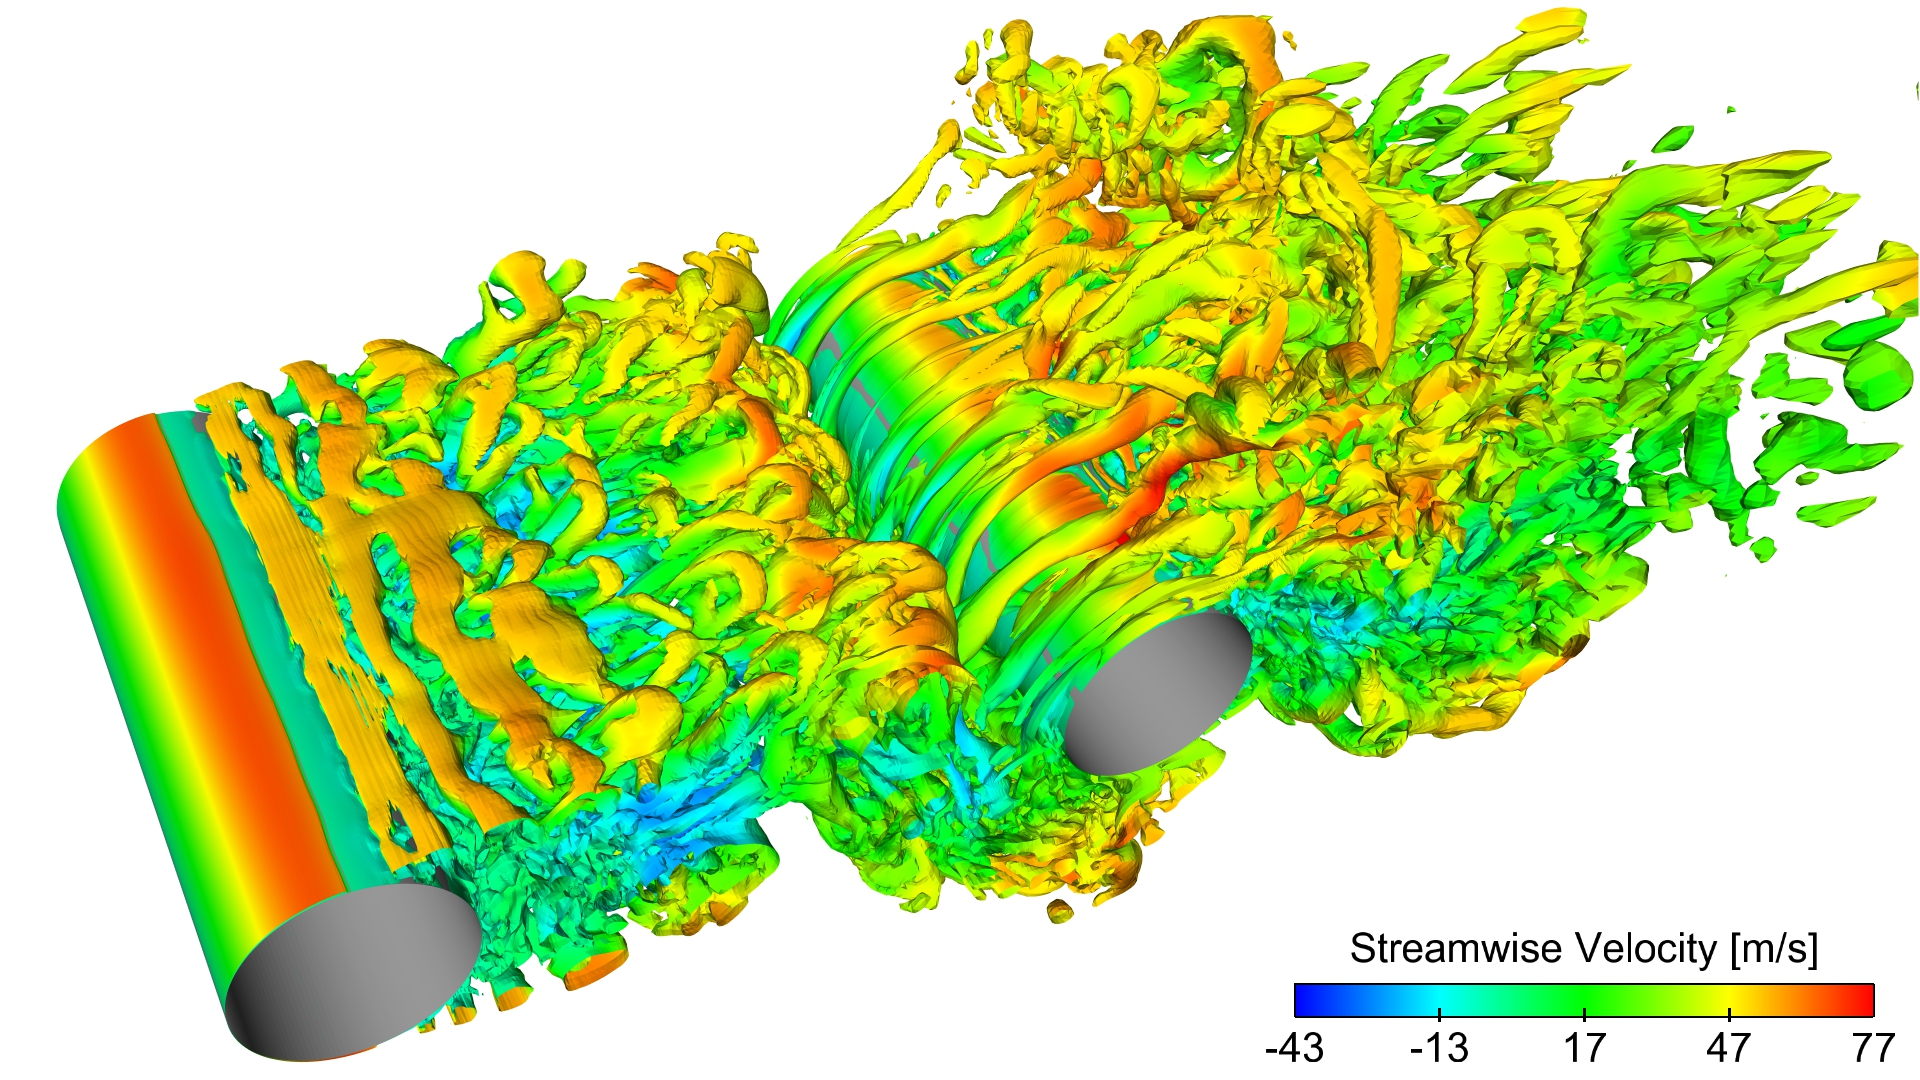
\includegraphics[width=0.40\textwidth]{tc_q_criteria}
	\bicaption{Q判据等值面图,同时测试一下一个很长的标题,比如这真的是一个很长很长很长很长很长很长很长很长的标题。}{Isocontour of Q criteria, at the same time, this is to test a long title, for instance, this is a really very long very long very long very long very long title.}
	\label{fig:tc_q_criteria}
\end{figure}

如果插图的空白区域过大,以图片\verb|shock_cyn|为例,自动裁剪如图\ref{fig:shock_cyn}。
\begin{figure}[!htbp]
	\centering
	%trim option's parameter order: left bottom right top
	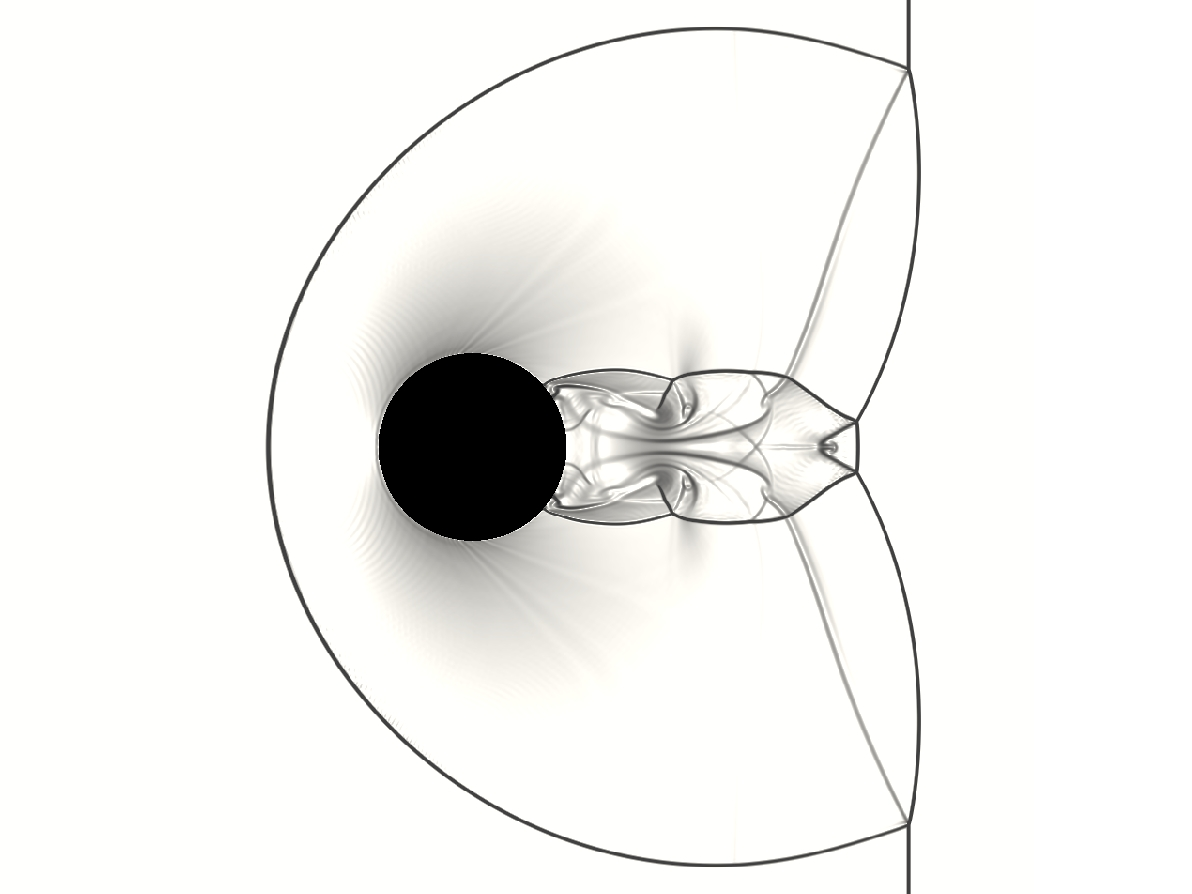
\includegraphics[trim = 30mm 0mm 30mm 0mm, clip, width=0.40\textwidth]{shock_cyn}
	\bicaption{激波圆柱作用。}{Shock-cylinder interaction.}
	\label{fig:shock_cyn}
\end{figure}

多图的插入如图\ref{fig:oaspl},多图不应在子图中给文本子标题,只要给序号,并在主标题中进行引用说明。
\begin{figure}[!htbp]
	\centering
	\begin{subfigure}[b]{0.35\textwidth}
		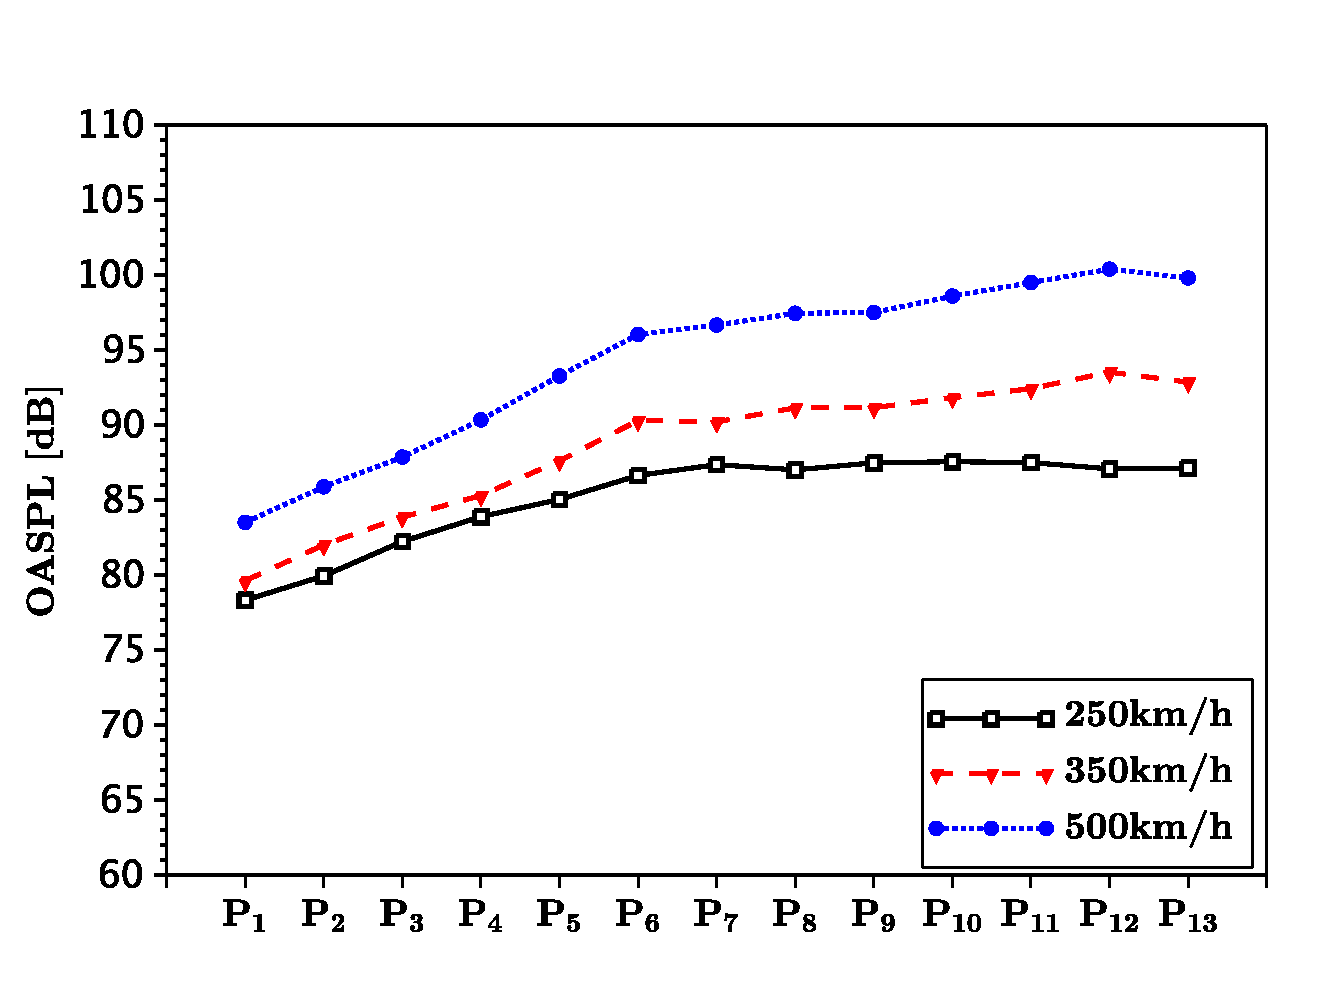
\includegraphics[width=\textwidth]{oaspl_a}
		\caption{}
		\label{fig:oaspl_a}
	\end{subfigure}%
	~% add desired spacing
	\begin{subfigure}[b]{0.35\textwidth}
		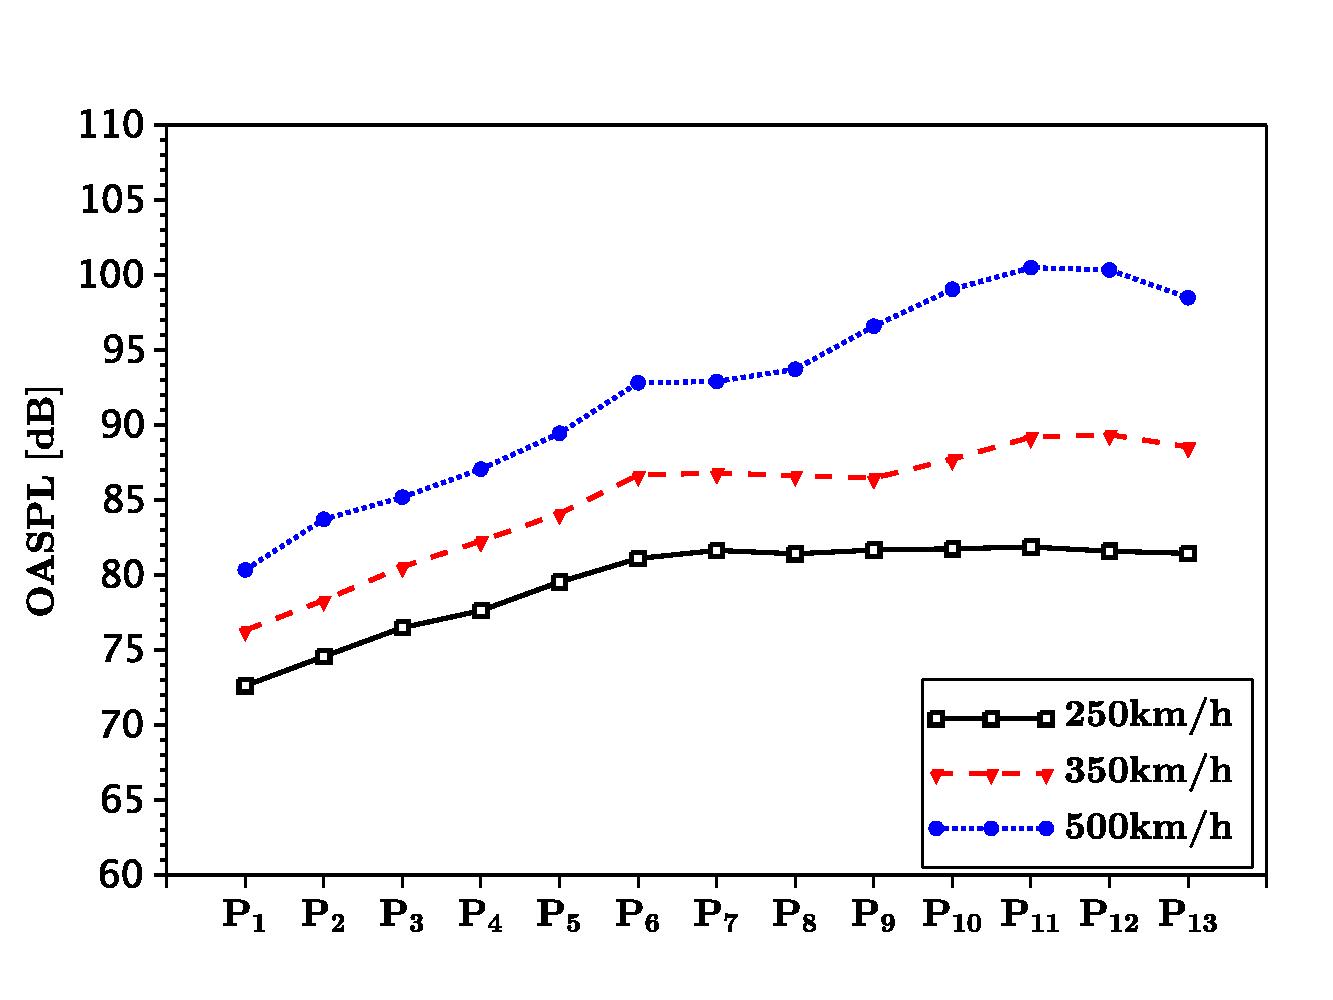
\includegraphics[width=\textwidth]{oaspl_b}
		\caption{}
		\label{fig:oaspl_b}
	\end{subfigure}
	\\% line break
	\begin{subfigure}[b]{0.35\textwidth}
		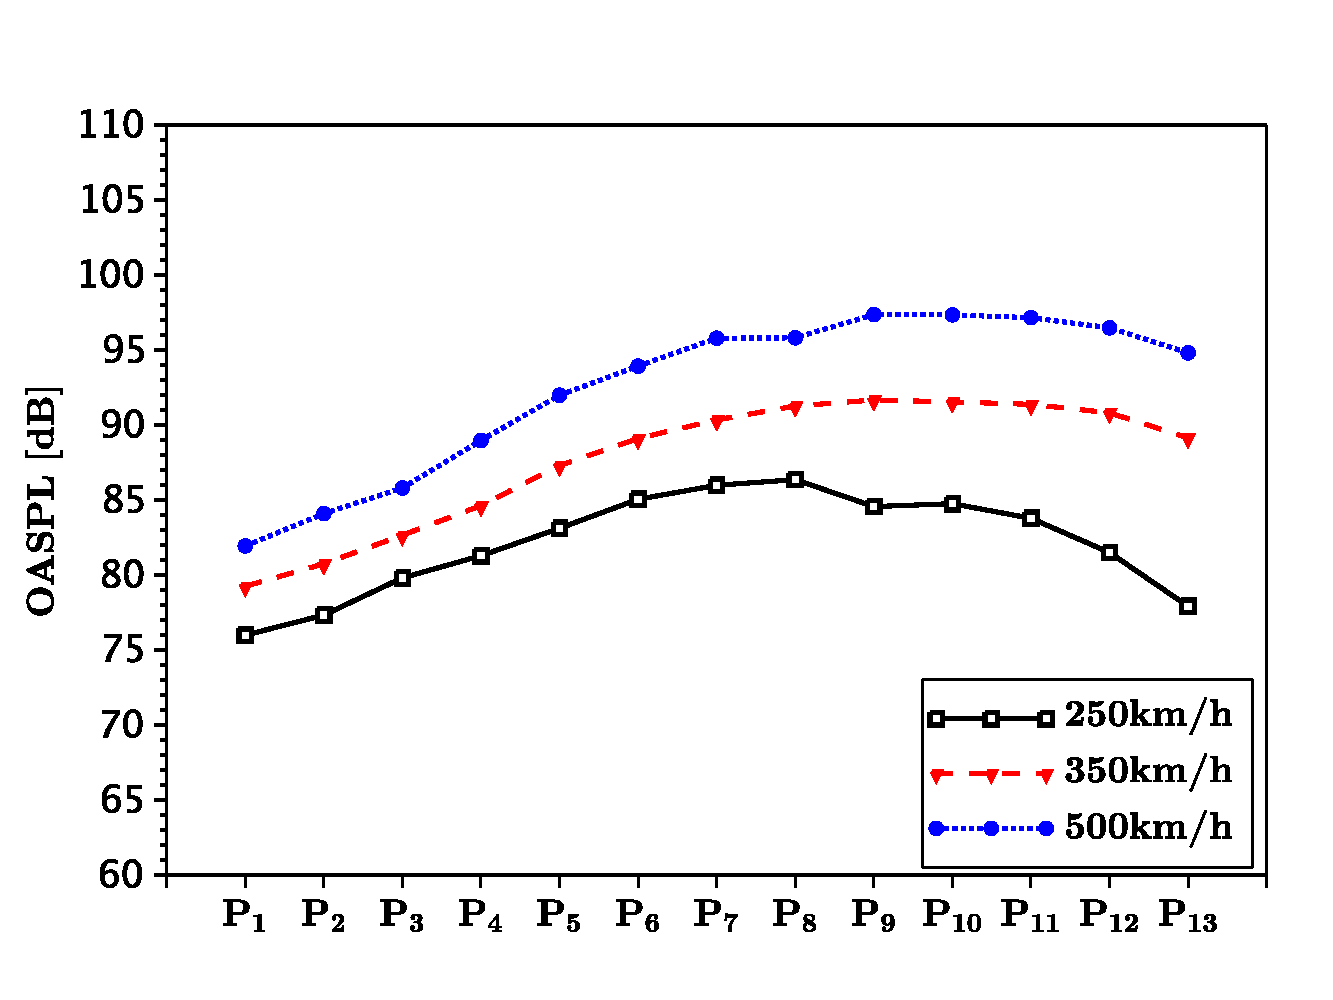
\includegraphics[width=\textwidth]{oaspl_c}
		\caption{}
		\label{fig:oaspl_c}
	\end{subfigure}%
	~% add desired spacing
	\begin{subfigure}[b]{0.35\textwidth}
		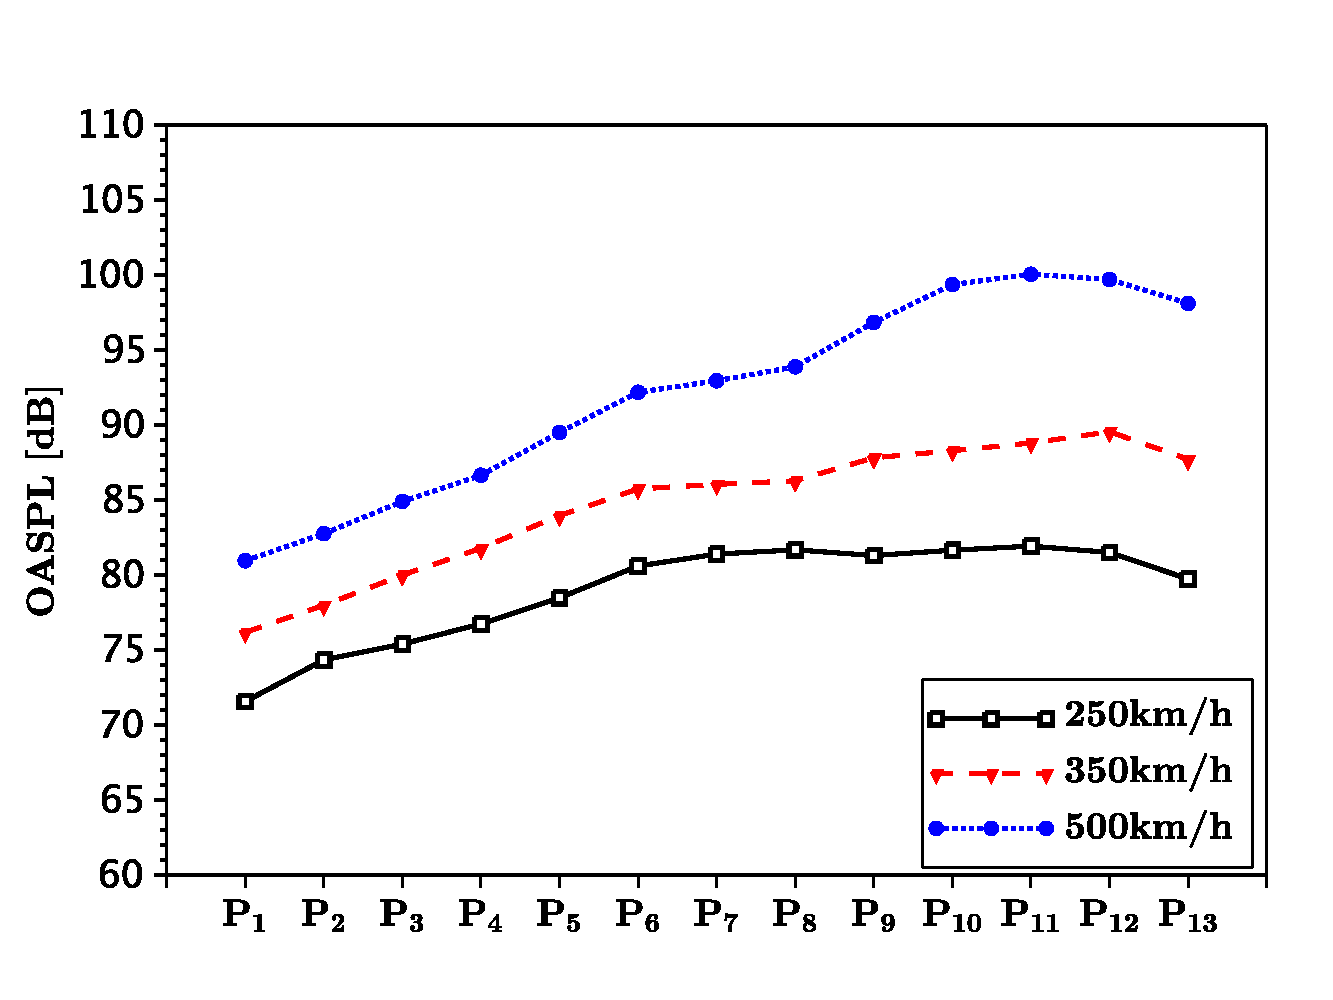
\includegraphics[width=\textwidth]{oaspl_d}
		\caption{}
		\label{fig:oaspl_d}
	\end{subfigure}
	\bicaption{总声压级。(a) 这是子图说明信息,(b) 这是子图说明信息,(c) 这是子图说明信息,(d) 这是子图说明信息。}{OASPL.(a) This is the explanation of subfig, (b) This is the explanation of subfig, (c) This is the explanation of subfig, (d) This is the explanation of subfig.}
	\label{fig:oaspl}
\end{figure}

\subsection{算法}

如见算法~\ref{alg:euclid},详细使用方法请参见文档 \href{https://ctan.org/pkg/algorithmicx?lang=en}{algorithmicx}。

\begin{algorithm}[!htbp]
	\small
	\caption{Euclid's algorithm}\label{alg:euclid}
	\begin{algorithmic}[1]
		\Procedure{Euclid}{$a,b$}\Comment{The g.c.d. of a and b}
		\State $r\gets a\bmod b$
		\While{$r\not=0$}\Comment{We have the answer if r is 0}
		\State $a\gets b$
		\State $b\gets r$
		\State $r\gets a\bmod b$
		\EndWhile\label{euclidendwhile}
		\State \textbf{return} $b$\Comment{The gcd is b}
		\EndProcedure
	\end{algorithmic}
\end{algorithm}

\subsection{参考文献引用}

参考文献引用过程以实例进行介绍,假设需要引用名为"Document Preparation System"的文献,步骤如下:

1)使用Google Scholar搜索Document Preparation System,在目标条目下点击Cite,展开后选择Import into BibTeX打开此文章的BibTeX索引信息,将它们copy添加到ref.bib文件中(此文件位于Biblio文件夹下)。

2)索引第一行 \verb|@article{lamport1986document,|中 \verb|lamport1986document| 即为此文献的label (\textbf{中文文献也必须使用英文label},一般遵照:姓氏拼音+年份+标题第一字拼音的格式),想要在论文中索引此文献,有两种索引类型:

文本类型:\verb|\citet{lamport1986document}|。正如此处所示 \citet{lamport1986document}; 

括号类型:\verb|\citep{lamport1986document}|。正如此处所示 \citep{lamport1986document}。

\textbf{多文献索引用英文逗号隔开}:

\verb|\citep{lamport1986document, chu2004tushu, chen2005zhulu}|。正如此处所示 \citep{lamport1986document, chu2004tushu, chen2005zhulu}

更多例子如:

\citet{walls2013drought} 根据 \citet{betts2005aging} 的研究,首次提出...。其中关于... \citep{walls2013drought, betts2005aging},是当前中国...得到迅速发展的研究领域 \citep{chen1980zhongguo, bravo1990comparative}。引用同一著者在同一年份出版的多篇文献时,在出版年份之后用
英文小写字母区别,如:\citep{yuan2012lana, yuan2012lanb, yuan2012lanc}。同一处引用多篇文献时,按出版年份由近及远依次标注,中间用
分号分开。例如 \citep{chen1980zhongguo, stamerjohanns2009mathml, hls2012jinji, niu2013zonghe}。

使用著者-出版年制(authoryear)式参考文献样式时,中文文献必须在BibTeX索引信息的 \textbf{key} 域(请参考ref.bib文件)填写作者姓名的拼音,才能使得文献列表按照拼音排序。参考文献表中的条目(不排序号),先按语种分类排列,语种顺 序是:中文、日文、英文、俄文、其他文种。然后,中文按汉语拼音字母顺序排列,日文按第一著者的姓氏笔画排序,西文和 俄文按第一著者姓氏首字母顺序排列。如中 \citep{niu2013zonghe}、日 \citep{Bohan1928}、英 \citep{stamerjohanns2009mathml}、俄 \citep{Dubrovin1906}。

如此,即完成了文献的索引,请查看下本文档的参考文献一章,看看是不是就是这么简单呢?是的,就是这么简单!

不同文献样式和引用样式,如著者-出版年制(authoryear)、顺序编码制(numbers)、上标顺序编码制(super)可在Thesis.tex中对artratex.sty调用实现,如:
\begin{itemize}
	\footnotesize
	\item \verb+\usepackage[numbers]{artratex}+ $\%$ 文本: Jones [1]; 括号: [1]
	\item \verb+\usepackage[super]{artratex}+ $\%$ 文本: Jones 上标[1]; 括号: 上标[1]
	\item \verb+\usepackage[authoryear]{artratex}+ $\%$ 文本: Jones (1995); 括号: (Jones, 1995)
	\item \verb+\usepackage[alpha]{artratex}+ $\%$ 文本: 不可用; 括号: [Jon95]
\end{itemize}

当前文档的默认参考文献样式为\textbf{authoryear}。若在上标(\textbf{super})模式下,希望在特定位置将上标改为嵌入式标,可使用

文本类型:\verb|\citetns{lamport1986document,chen2005zhulu}|。

正如此处所示 \citetns{lamport1986document,chen2005zhulu}

括号类型:\verb|\citepns{lamport1986document,chen2005zhulu}|。

正如此处所示 \citepns{lamport1986document,chen2005zhulu}

参考文献索引更为详细的信息,请见 \href{https://en.wikibooks.org/wiki/LaTeX/Bibliography_Management}{WiKibook Bibliography}。\nocite{*}% 使文献列表显示所有参考文献(包括未引用文献)

\section{常见使用问题}\label{sec:qa}

\begin{itemize}
	\item 模板每次发布前,都已在Windows,Linux,MacOS系统上测试通过。下载模板后,若编译出现错误,则请见 \href{https://github.com/mohuangrui/ucasthesis/wiki}{ucasthesis知识小站} 的 \href{https://github.com/mohuangrui/ucasthesis/wiki/%E7%BC%96%E8%AF%91%E6%8C%87%E5%8D%97}{编译指南}。
		
		\item 模板文档的编码为UTF-8编码。所有文件都必须采用UTF-8编码,否则编译后生成的文档将出现乱码文本。若出现文本编辑器无法打开文档或打开文档乱码的问题,请检查编辑器对UTF-8编码的支持。如果使用WinEdt作为文本编辑器(\textbf{不推荐使用}),应在其Options -> Preferences -> wrapping选项卡下将两种Wrapping Modes中的内容:
		
		TeX;HTML;ANSI;ASCII|DTX...
		
		修改为:TeX;\textbf{UTF-8|ACP;}HTML;ANSI;ASCII|DTX...
		
		同时,取消Options -> Preferences -> Unicode中的Enable ANSI Format。
		
		\item 推荐选择xelatex或lualatex编译引擎编译中文文档。编译脚本的默认设定为xelatex编译引擎。你也可以选择不使用脚本编译,如直接使用 \LaTeX{}文本编辑器编译。注:\LaTeX{}文本编辑器编译的默认设定为pdflatex编译引擎,若选择xelatex或lualatex编译引擎,请进入下拉菜单选择。为正确生成引用链接,需要进行全编译。
		
		\item Texmaker使用简介
		\begin{itemize}
			\footnotesize
			\item 使用 Texmaker “打开 (Open)” Thesis.tex。
			\item 菜单 “选项 (Options)” -> “设置当前文档为主文档 (Define as Master Document)”
			\item 菜单 “自定义 (User)” -> “自定义命令 (User Commands)” -> “编辑自定义命令 (Edit User Commands)” -> 左侧选择 “command 1”,右侧 “菜单项 (Menu Item)” 填入 Auto Build -> 点击下方“向导 (Wizard)” -> “添加 (Add)”: xelatex + bibtex + xelatex + xelatex + pdf viewer -> 点击“完成 (OK)”
			\item 使用 Auto Build 编译带有未生成引用链接的源文件,可以仅使用 xelatex 编译带有已经正确生成引用链接的源文件。
			\item 编译完成,“查看(View)” PDF,在PDF中 “ctrl+click” 可链接到相对应的源文件。
		\end{itemize}
		
		\item 模版的设计可能地考虑了适应性。致谢等所有条目都是通过最为通用的
		
		\verb+\chapter{item name}+  and \verb+\section*{item name}+
		
		来显式实现的 (请观察Backmatter.tex),从而可以随意添加,放置,和修改,如同一般章节。对于图表目录名称则可在ucasthesis.cfg中进行修改。
		
		\item 设置文档样式: 在artratex.sty中搜索关键字定位相应命令,然后修改
		\begin{itemize}
			\item 正文行距:启用和设置 \verb|\linespread{1.5}|,默认1.5倍行距。
			\item 参考文献行距:修改 \verb|\setlength{\bibsep}{0.0ex}|
			\item 目录显示级数:修改 \verb|\setcounter{tocdepth}{2}|
			\item 文档超链接的颜色及其显示:修改 \verb|\hypersetup|
		\end{itemize}
		
		\item 文档内字体切换方法:
		\begin{itemize}
			\item 宋体:国科大论文模板ucasthesis 或 \textrm{国科大论文模板ucasthesis}
			\item 粗宋体:{\bfseries 国科大论文模板ucasthesis} 或 \textbf{国科大论文模板ucasthesis}
			\item 黑体:{\sffamily 国科大论文模板ucasthesis} 或 \textsf{国科大论文模板ucasthesis}
			\item 粗黑体:{\bfseries\sffamily 国科大论文模板ucasthesis} 或 \textsf{\bfseries 国科大论文模板ucasthesis}
			\item 仿宋:{\ttfamily 国科大论文模板ucasthesis} 或 \texttt{国科大论文模板ucasthesis}
			\item 粗仿宋:{\bfseries\ttfamily 国科大论文模板ucasthesis} 或 \texttt{\bfseries 国科大论文模板ucasthesis}
			\item 楷体:{\itshape 国科大论文模板ucasthesis} 或 \textit{国科大论文模板ucasthesis}
			\item 粗楷体:{\bfseries\itshape 国科大论文模板ucasthesis} 或 \textit{\bfseries 国科大论文模板ucasthesis}
		\end{itemize}
		
		\item 封面下划线上的文本不居中下划线,这是因为下划线前面还有字头,导致文本只能在页面居中和在下划线上居中二选一。当前封面采取页面居中。如需要调整文本在下划线上的位置,可用 \verb|\hspace*{+/- n.0em}| 命令来插入或删除 n 个空格,进行手动调整,比如
		
		\verb|\advisor{\hspace*{+3.0em} xxx~研究员~xxx单位}|
		
		有时下划线看上去粗细不一致,这是显示的问题,打印正常。
	\end{itemize}
	
	


\chapter{撰写要求及说明}
\vbox{}\vbox{}
\section{撰写要求}
学位论文是研究生科研工作成果的集中体现,是评判学位申请者学术水平、授予其学位的主要依据,是科研领域重要的文献资料。根据《科学技术报告、学位论文和学术论文的编写格式》(GB/T 7713-1987)、《学位论文编写规则》(GB/T 7713.1-2006)和《文后参考文献著录规则》(GB7714—87)等国家有关标准,特制订本规定。

\section{论文封面设置}
此模板暂时未能实现封面格式的封装,因此需要单独制作封面并导入到\LaTeX{}中。具体制作方法为,在Word中制作好封面以后打印完PDF文件,再将PDF文件导入到\LaTeX{}即可。在源文件中已有fengmian.doc文件,在使用过程中只需要打开此文档填入自己的论文信息即可,随后使用虚拟打印机打印为fengmian.pdf文件(导入代码已设置完毕,无需关心导入)保存即可(建议使用adobe printer打印)。

正文中其它的文件格式已按照温大硕士毕业论文Word模板设置完毕,因此在使用该软件的过程中无需关心格式,只需关心文档的写作即可,因为\LaTeX{}的主要优势除了生成高质量的PDF文件以外,另一大优势就是格式文档分离。


\section{测试生僻字}

霜蟾盥薇曜灵霜颸妙鬘虚霩淩澌菀枯菡萏泬寥窅冥毰毸濩落霅霅便嬛岧峣瀺灂姽婳愔嫕飒纚棽俪緸冤莩甲摛藻卮言倥侗椒觞期颐夜阑彬蔚倥偬澄廓簪缨陟遐迤逦缥缃鹣鲽憯懔闺闼璀错媕婀噌吰澒洞阛闠覼缕玓瓑逡巡諓諓琭琭瀌瀌踽踽叆叇氤氲瓠犀流眄蹀躞赟嬛茕頔璎珞螓首蘅皋惏悷缱绻昶皴皱颟顸愀然菡萏卑。

暒墌墍墎墏墐墒墒墓墔墕墖墘墖墚墛坠墝增墠墡墢墣墤墥墦墧墨墩墪樽墬墭堕墯墰墱墲坟墴墵垯墷墸墹墺墙墼墽垦墿壀壁壂壃壄壅壆坛壈壉壊垱壌壍埙壏壐壑壒压壔壕壖壗垒圹垆壛壜壝垄壠壡坜壣壤壥壦壧壨坝塆圭嫶嫷嫸嫹嫺娴嫼嫽嫾婳妫嬁嬂嬃嬄嬅嬆嬇娆嬉嬊娇嬍嬎嬏嬐嬑嬒嬓嬔嬕嬖嬗嬘嫱嬚嬛嬜嬞嬟嬠嫒嬢嬣嬥嬦嬧嬨嬩嫔嬫嬬奶嬬嬮嬯婴嬱嬲嬳嬴嬵嬶嬷婶嬹嬺嬻嬼嬽嬾嬿孀孁孂娘孄孅孆孇孆孈孉孊娈孋孊孍孎孏嫫婿媚嵭嵮嵯嵰嵱嵲嵳嵴嵵嵶嵷嵸嵹嵺嵻嵼嵽嵾嵿嶀嵝嶂嶃崭嶅嶆岖嶈嶉嶊嶋嶌嶍嶎嶏嶐嶑嶒嶓嵚嶕嶖嶘嶙嶚嶛嶜嶝。

嶞嶟峤嶡峣嶣嶤嶥嶦峄峃嶩嶪嶫嶬嶭崄嶯嶰嶱嶲嶳岙嶵嶶嶷嵘嶹岭嶻屿岳帋巀巁巂巃巄巅巆巇巈巉巊岿巌巍巎巏巐巑峦巓巅巕岩巗巘巙巚帠帡帢帣帤帨帩帪帬帯帰帱帲帴帵帷帹帺帻帼帽帾帿幁幂帏幄幅幆幇幈幉幊幋幌幍幎幏幐幑幒幓幖幙幚幛幜幝幞帜幠幡幢幤幥幦幧幨幩幪幭幮幯幰幱庍庎庑庖庘庛庝庠庡庢庣庤庥庨庩庪庬庮庯庰庱庲庳庴庵庹庺庻庼庽庿廀厕廃厩廅廆廇廋廌廍庼廏廐廑廒廔廕廖廗廘廙廛廜廞庑廤廥廦廧廨廭廮廯廰痈廲廵廸廹廻廼廽廿弁弅弆弇弉弖弙弚弜弝弞弡弢弣弤弨弩弪弫弬弭弮弰弲弪弴弶弸弻弼弽弿彖彗彘彚。

%\input{Tex/Chap_5}
%\input{Tex/Chap_6}
%---------------------------------------------------------------------------%
% main content
%-
%-> Appendix
%-
%\cleardoublepage%
%\appendix% initialize the environment
%\chapter{撰写要求及说明}
\vbox{}\vbox{}
\section{撰写要求}
学位论文是研究生科研工作成果的集中体现,是评判学位申请者学术水平、授予其学位的主要依据,是科研领域重要的文献资料。根据《科学技术报告、学位论文和学术论文的编写格式》(GB/T 7713-1987)、《学位论文编写规则》(GB/T 7713.1-2006)和《文后参考文献著录规则》(GB7714—87)等国家有关标准,特制订本规定。

\section{论文封面设置}
此模板暂时未能实现封面格式的封装,因此需要单独制作封面并导入到\LaTeX{}中。具体制作方法为,在Word中制作好封面以后打印完PDF文件,再将PDF文件导入到\LaTeX{}即可。在源文件中已有fengmian.doc文件,在使用过程中只需要打开此文档填入自己的论文信息即可,随后使用虚拟打印机打印为fengmian.pdf文件(导入代码已设置完毕,无需关心导入)保存即可(建议使用adobe printer打印)。

正文中其它的文件格式已按照温大硕士毕业论文Word模板设置完毕,因此在使用该软件的过程中无需关心格式,只需关心文档的写作即可,因为\LaTeX{}的主要优势除了生成高质量的PDF文件以外,另一大优势就是格式文档分离。


\section{测试生僻字}

霜蟾盥薇曜灵霜颸妙鬘虚霩淩澌菀枯菡萏泬寥窅冥毰毸濩落霅霅便嬛岧峣瀺灂姽婳愔嫕飒纚棽俪緸冤莩甲摛藻卮言倥侗椒觞期颐夜阑彬蔚倥偬澄廓簪缨陟遐迤逦缥缃鹣鲽憯懔闺闼璀错媕婀噌吰澒洞阛闠覼缕玓瓑逡巡諓諓琭琭瀌瀌踽踽叆叇氤氲瓠犀流眄蹀躞赟嬛茕頔璎珞螓首蘅皋惏悷缱绻昶皴皱颟顸愀然菡萏卑。

暒墌墍墎墏墐墒墒墓墔墕墖墘墖墚墛坠墝增墠墡墢墣墤墥墦墧墨墩墪樽墬墭堕墯墰墱墲坟墴墵垯墷墸墹墺墙墼墽垦墿壀壁壂壃壄壅壆坛壈壉壊垱壌壍埙壏壐壑壒压壔壕壖壗垒圹垆壛壜壝垄壠壡坜壣壤壥壦壧壨坝塆圭嫶嫷嫸嫹嫺娴嫼嫽嫾婳妫嬁嬂嬃嬄嬅嬆嬇娆嬉嬊娇嬍嬎嬏嬐嬑嬒嬓嬔嬕嬖嬗嬘嫱嬚嬛嬜嬞嬟嬠嫒嬢嬣嬥嬦嬧嬨嬩嫔嬫嬬奶嬬嬮嬯婴嬱嬲嬳嬴嬵嬶嬷婶嬹嬺嬻嬼嬽嬾嬿孀孁孂娘孄孅孆孇孆孈孉孊娈孋孊孍孎孏嫫婿媚嵭嵮嵯嵰嵱嵲嵳嵴嵵嵶嵷嵸嵹嵺嵻嵼嵽嵾嵿嶀嵝嶂嶃崭嶅嶆岖嶈嶉嶊嶋嶌嶍嶎嶏嶐嶑嶒嶓嵚嶕嶖嶘嶙嶚嶛嶜嶝。

嶞嶟峤嶡峣嶣嶤嶥嶦峄峃嶩嶪嶫嶬嶭崄嶯嶰嶱嶲嶳岙嶵嶶嶷嵘嶹岭嶻屿岳帋巀巁巂巃巄巅巆巇巈巉巊岿巌巍巎巏巐巑峦巓巅巕岩巗巘巙巚帠帡帢帣帤帨帩帪帬帯帰帱帲帴帵帷帹帺帻帼帽帾帿幁幂帏幄幅幆幇幈幉幊幋幌幍幎幏幐幑幒幓幖幙幚幛幜幝幞帜幠幡幢幤幥幦幧幨幩幪幭幮幯幰幱庍庎庑庖庘庛庝庠庡庢庣庤庥庨庩庪庬庮庯庰庱庲庳庴庵庹庺庻庼庽庿廀厕廃厩廅廆廇廋廌廍庼廏廐廑廒廔廕廖廗廘廙廛廜廞庑廤廥廦廧廨廭廮廯廰痈廲廵廸廹廻廼廽廿弁弅弆弇弉弖弙弚弜弝弞弡弢弣弤弨弩弪弫弬弭弮弰弲弪弴弶弸弻弼弽弿彖彗彘彚。
% appendix content
%-
%-> Backmatter: bibliography, glossary, index
%-
\backmatter% initialize the environment
%-
%\appendix% initialize the environment  ------如果要求附录在参考文献前面,则打开这个开关
%\chapter{撰写要求及说明}
\vbox{}\vbox{}
\section{撰写要求}
学位论文是研究生科研工作成果的集中体现,是评判学位申请者学术水平、授予其学位的主要依据,是科研领域重要的文献资料。根据《科学技术报告、学位论文和学术论文的编写格式》(GB/T 7713-1987)、《学位论文编写规则》(GB/T 7713.1-2006)和《文后参考文献著录规则》(GB7714—87)等国家有关标准,特制订本规定。

\section{论文封面设置}
此模板暂时未能实现封面格式的封装,因此需要单独制作封面并导入到\LaTeX{}中。具体制作方法为,在Word中制作好封面以后打印完PDF文件,再将PDF文件导入到\LaTeX{}即可。在源文件中已有fengmian.doc文件,在使用过程中只需要打开此文档填入自己的论文信息即可,随后使用虚拟打印机打印为fengmian.pdf文件(导入代码已设置完毕,无需关心导入)保存即可(建议使用adobe printer打印)。

正文中其它的文件格式已按照温大硕士毕业论文Word模板设置完毕,因此在使用该软件的过程中无需关心格式,只需关心文档的写作即可,因为\LaTeX{}的主要优势除了生成高质量的PDF文件以外,另一大优势就是格式文档分离。


\section{测试生僻字}

霜蟾盥薇曜灵霜颸妙鬘虚霩淩澌菀枯菡萏泬寥窅冥毰毸濩落霅霅便嬛岧峣瀺灂姽婳愔嫕飒纚棽俪緸冤莩甲摛藻卮言倥侗椒觞期颐夜阑彬蔚倥偬澄廓簪缨陟遐迤逦缥缃鹣鲽憯懔闺闼璀错媕婀噌吰澒洞阛闠覼缕玓瓑逡巡諓諓琭琭瀌瀌踽踽叆叇氤氲瓠犀流眄蹀躞赟嬛茕頔璎珞螓首蘅皋惏悷缱绻昶皴皱颟顸愀然菡萏卑。

暒墌墍墎墏墐墒墒墓墔墕墖墘墖墚墛坠墝增墠墡墢墣墤墥墦墧墨墩墪樽墬墭堕墯墰墱墲坟墴墵垯墷墸墹墺墙墼墽垦墿壀壁壂壃壄壅壆坛壈壉壊垱壌壍埙壏壐壑壒压壔壕壖壗垒圹垆壛壜壝垄壠壡坜壣壤壥壦壧壨坝塆圭嫶嫷嫸嫹嫺娴嫼嫽嫾婳妫嬁嬂嬃嬄嬅嬆嬇娆嬉嬊娇嬍嬎嬏嬐嬑嬒嬓嬔嬕嬖嬗嬘嫱嬚嬛嬜嬞嬟嬠嫒嬢嬣嬥嬦嬧嬨嬩嫔嬫嬬奶嬬嬮嬯婴嬱嬲嬳嬴嬵嬶嬷婶嬹嬺嬻嬼嬽嬾嬿孀孁孂娘孄孅孆孇孆孈孉孊娈孋孊孍孎孏嫫婿媚嵭嵮嵯嵰嵱嵲嵳嵴嵵嵶嵷嵸嵹嵺嵻嵼嵽嵾嵿嶀嵝嶂嶃崭嶅嶆岖嶈嶉嶊嶋嶌嶍嶎嶏嶐嶑嶒嶓嵚嶕嶖嶘嶙嶚嶛嶜嶝。

嶞嶟峤嶡峣嶣嶤嶥嶦峄峃嶩嶪嶫嶬嶭崄嶯嶰嶱嶲嶳岙嶵嶶嶷嵘嶹岭嶻屿岳帋巀巁巂巃巄巅巆巇巈巉巊岿巌巍巎巏巐巑峦巓巅巕岩巗巘巙巚帠帡帢帣帤帨帩帪帬帯帰帱帲帴帵帷帹帺帻帼帽帾帿幁幂帏幄幅幆幇幈幉幊幋幌幍幎幏幐幑幒幓幖幙幚幛幜幝幞帜幠幡幢幤幥幦幧幨幩幪幭幮幯幰幱庍庎庑庖庘庛庝庠庡庢庣庤庥庨庩庪庬庮庯庰庱庲庳庴庵庹庺庻庼庽庿廀厕廃厩廅廆廇廋廌廍庼廏廐廑廒廔廕廖廗廘廙廛廜廞庑廤廥廦廧廨廭廮廯廰痈廲廵廸廹廻廼廽廿弁弅弆弇弉弖弙弚弜弝弞弡弢弣弤弨弩弪弫弬弭弮弰弲弪弴弶弸弻弼弽弿彖彗彘彚。
% appendix content
%-
\intotoc{\bibname}% add link to contents table and bookmark
%\begin{thebibliography}{113}
	\providecommand{\natexlab}[1]{#1}
	\providecommand{\url}[1]{#1}
	\providecommand{\href}[2]{\url{#2}}
	\providecommand{\doi}[1]{DOI: \href{http://dx.doi.org/#1}{#1}}
	\expandafter\ifx\csname urlstyle\endcsname\relax\relax\else
	\urlstyle{same}\fi
	\vbox{}
	\vbox{}

	\bibitem{bennett1993teleporting}
	Bennett C~H, Brassard G, Cr{\'e}peau C, et~al.
	\newblock Teleporting an unknown quantum state via dual classical and
	einstein-podolsky-rosen channels\allowbreak[J].
	\newblock Phys. Rev. L, 1993, 70\penalty0 (13): 1895-1899.
	
	\bibitem[Bennett\ et~al.(1992)Bennett and Wiesner]{bennett1992communication}
	Bennett C~H, Wiesner S~J.
	\newblock Communication via one-and two-particle operators on
	einstein-podolsky-rosen states\allowbreak[J].
	\newblock Phys. Rev. L, 1992, 69\penalty0 (20): 2881-2884.
	
	\bibitem[Bennett\ et~al.(1984)Bennett and Brassard]{bennett1984proceedings}
	Bennett C~H, Brassard G.
	\newblock Proceedings of the ieee international conference on computers,
	systems and signal processing, bangalore, india\allowbreak[Z].
	 IEEE New York, 1984.
	
	\bibitem[Beige\ et~al.(2001)Beige, Englert, Kurtsiefer, and
	Weinfurter]{beige2001secure}
	Beige A, Englert B~G, Kurtsiefer C, et~al.
	\newblock Secure communication with a publicly known key\allowbreak[J].
	\newblock arXiv preprint quant-ph/0111106, 2001.
	
	\bibitem[Shor(1994)]{shor1994proc}
	Shor P.
	\newblock Proc. 35th annual symp. foundations of computer
	science\allowbreak[Z]. IEEE Computer Society Press Los Alomitos, CA, 1994.
	
	\bibitem[Nielsen\ et~al.(2002)Nielsen and Chuang]{nielsen2002quantum}
	Nielsen M~A, Chuang I.
	\newblock Quantum computation and quantum information\allowbreak[Z]. AAPT, 2002.
	
	\bibitem[Ekert\ et~al.(1996)Ekert and Jozsa]{ekert1996quantum}
	kert A, Jozsa R.
	\newblock Quantum computation and shor's factoring algorithm\allowbreak[J].
	\newblock Reviews of Modern Physics, 1996, 68\penalty0 (3): 733-753.
	
	\bibitem[Einstein\ et~al.(1935)Einstein, Podolsky, and Rosen]{einstein1935can}
	Einstein A, Podolsky B, Rosen N.
	\newblock Can quantum-mechanical description of physical reality be considered
	complete?\allowbreak[J].
	\newblock Physical review, 1935, 47\penalty0 (10): 777-780.
	
	\bibitem[Schrödinger(1935)]{article1935}
	Schrödinger E.
	\newblock Die gegenwärtige situation in der quantenmechanik\allowbreak[J].
	\newblock Naturwissenschaften, 1935, 23: 807-812.
	
	\bibitem[Bell(1964{\natexlab{a}})]{Bell}
	Bell J~S.
	\newblock On the einstein podolsky rosen paradox\allowbreak[J].
	\newblock Physics, 1964, 1\penalty0 (6): 195--200.
	
	\bibitem[K.~Wootters(1997)]{article1997}
	K.~Wootters W.
	\newblock Entanglement of formation of an arbitrary state of two
	qubits\allowbreak[J].
	\newblock Physical Review Letters, 1998, 80(10): 2245--2254.
	
	\bibitem[Wang\ et~al.(2003)Wang and Sanders]{PhysRevA.68.012101}
	Wang X, Sanders B~C.
	\newblock Spin squeezing and pairwise entanglement for symmetric multiqubit
	states\allowbreak[J].
	\newblock Phys. Rev. A, 2003, 68(1): 012101--01216.
	
	\bibitem[Kennard(1927)]{Kennard1927}
	Kennard E~H.
	\newblock Zur quantenmechanik einfacher bewegungstypen\allowbreak[J].
	\newblock Zeitschrift f{\"u}r Physik, 1927, 44\penalty0 (4): 326--352.
	
	\bibitem[Stoler(1970)]{stoler1970equivalence}
	Stoler D.
	\newblock Equivalence classes of minimum uncertainty packets\allowbreak[J].
	\newblock Phys. Rev. D, 1970, 1(12): 3217--3288.
	
	\bibitem[Yuen(1976)]{yuen1976two}
	Yuen H~P.
	\newblock Two-photon coherent states of the radiation field\allowbreak[J].
	\newblock Phys. Rev. A, 1976, 13(6): 2226--2231.
	
	\bibitem[Walls\ et~al.(1981)Walls and Zoller]{PhysRevLett.47.709}
	Walls D~F, Zoller P.
	\newblock Reduced quantum fluctuations in resonance fluorescence\allowbreak[J].
	\newblock Phys. Rev. Lett., 1981, 47: 709--711.
	
	\bibitem[Wineland\ et~al.(1992)Wineland, Bollinger, Itano, Moore, and
	Heinzen]{PRA1992Wineland}
	Wineland D~J, ollinger J~J, Itano W~M, et~al.
	\newblock Spin squeezing and reduced quantum noise in
	spectroscopy\allowbreak[J].
	\newblock Phys. Rev. A, 1992, 46: R6797--R6800.
	
	\bibitem[M.Kitagawa\ et~al.(1993)M.Kitagawa and M.Ueda]{PRA1993Kitagawa}
	M.Kitagawa, M.Ueda.
	\newblock Squeezed spin states\allowbreak[J].
	\newblock Phys. Rev. Lett, 1993, 47: 5138--5143.
	
	\bibitem[S\o{}rensen\ et~al.(2002)S\o{}rensen and M\o{}lmer]{PRA2002SS}
	S\o{}rensen A~S, M\o{}lmer K.
	\newblock Entangling atoms in bad cavities\allowbreak[J].
	\newblock Phys. Rev. A, 2002, 66(2): 022314-022321.
	
	\bibitem[Louchet-Chauvet A, Appel J, Renema J J, et al.(2010)Louchet-Chauvet A, Appel J, Renema J J, et al.]{LCA2010}
	Louchet-Chauvet A, Appel J, Renema J J, et al.
	\newblock Entanglement-assisted atomic clock beyond the projection noise limit\allowbreak[J].
	\newblock New Journal of Physics, 2010, 12(6): 065032.
		
	\bibitem[Borregaard\ et~al.(2017)Borregaard, Davis, Bentsen, Schleier-Smith,
	and S?rensen]{NJP2017J-Borregaard}
	Borregaard J, Davis E~J, Bentsen G~S, et~al.
	\newblock One- and two-axis squeezing of atomic ensembles in optical
	cavities\allowbreak[J].
	\newblock New Journal of Physics, 2017, 19\penalty0 (9): 093021.
	
	\bibitem[Orzel\ et~al.(2001)Orzel, Tuchman, Fenselau, Yasuda, and
	Kasevich]{orzel2001squeezed}
	Orzel C, Tuchman A, Fenselau M, et~al.
	\newblock Squeezed states in a bose-einstein condensate\allowbreak[J].
	\newblock Science, 2001, 291\penalty0 (5512): 2386--2389.
	
	\bibitem[Hald\ et~al.(1999)Hald, S{\o}rensen, Schori, and Polzik]{hald1999spin}
	Hald J, S{\o}rensen J, Schori C, et~al.
	\newblock Spin squeezed atoms: a macroscopic entangled ensemble created by
	light\allowbreak[J].
	\newblock Phys. Rev. L, 1999, 83\penalty0 (7): 1319--1925.
	
	\bibitem[Riedel\ et~al.(2010)Riedel, B{\"o}hi, Li, H{\"a}nsch, Sinatra, and
	Treutlein]{riedel2010atom}
	Riedel M~F, B{\"o}hi P, Li Y, et~al.
	\newblock Atom-chip-based generation of entanglement for quantum
	metrology\allowbreak[J].
	\newblock Nature, 2010, 464\penalty0 (7292): 1170.
	
	\bibitem[Appel\ et~al.(2009)Appel, Windpassinger, Oblak, Hoff, Kj{\ae}rgaard,
	and Polzik]{appel2009mesoscopic}
	Appel J, Windpassinger P~J, Oblak D, et~al.
	\newblock Mesoscopic atomic entanglement for precision measurements beyond the
	standard quantum limit\allowbreak[J].
	\newblock Proceedings of the National Academy of Sciences, 2009, 106\penalty0
	(27): 10960--10965.
	
	\bibitem[Stolze\ et~al.(2008)Stolze and Suter]{stolze2008quantum}
	Stolze J, Suter D.
	\newblock Quantum computing: a short course from theory to
	experiment\allowbreak[M]. John Wiley \& Sons, 2008.
	
	\bibitem[Oblak\ et~al.(2005)Oblak, Petrov, Alzar, Tittel, Vershovski,
	Mikkelsen, S{\o}rensen, and Polzik]{oblak2005quantum}
	Oblak D, etrov P~G, Alzar C~L~G, et~al.
	\newblock Quantum-noise-limited interferometric measurement of atomic noise:
	Towards spin squeezing on the cs clock transition\allowbreak[J].
	\newblock Phys. Rev. A, 2005, 71\penalty0 (4): 043807--043819.
	
	\bibitem[Meyer\ et~al.(2001)Meyer, Rowe, Kielpinski, Sackett, Itano, Monroe,
	and Wineland]{meyer2001experimental}
	Meyer V, Rowe M, Kielpinski D, et~al.
	\newblock Experimental demonstration of entanglement-enhanced rotation angle
	estimation using trapped ions\allowbreak[J].
	\newblock Phys. Rev. L, 2001, 86\penalty0 (26): 5870--5895.
	
	\bibitem[Goda\ et~al.(2008)Goda, Miyakawa, Mikhailov, Saraf, Adhikari,
	McKenzie, Ward, Vass, Weinstein, and Mavalvala]{goda2008quantum}
	Goda K, Miyakawa O, Mikhailov E~E, et~al.
	\newblock A quantum-enhanced prototype gravitational-wave
	detector\allowbreak[J].
	\newblock Nature Physics, 2008, 4\penalty0 (6): 472--479.
	
	\bibitem[Scully\ et~al.(1999)Scully and Zubairy]{scully1999quantum}
	Scully M~O, Zubairy M~S.
	\newblock Quantum optics\allowbreak[Z]. AAPT, 1999.
	
	\bibitem[Pennarun\ et~al.(2007)Pennarun, Bradley, and
	Olsen]{pennarun2007tripartite}
	Pennarun C, Bradley A, OLSEN M.
	\newblock Tripartite entanglement and threshold properties of coupled
	intracavity down-conversion and sum-frequency generation\allowbreak[J].
	\newblock Phys. Rev. A, 2007, 76\penalty0 (6): 063812--063819.
	
	\bibitem[CC-Tannoudji(1998)]{cc1998roc}
	C C-Tannoudji J.
	\newblock Roc, and G. Grynberg, atom-photon interactions\allowbreak[Z]. Wiley, New York, 1998.
	
	\bibitem[Griffiths(2005)]{griffiths2005introduction}
	Griffiths D~J.
	\newblock Introduction to electrodynamics\allowbreak[Z]. AAPT, 2005.
	
	\bibitem[Rabi(1937)]{rabi1937space}
	Rabi I~I.
	\newblock Space quantization in a gyrating magnetic field\allowbreak[J].
	\newblock Physical Review, 1937, 51\penalty0 (8): 652--659.
	
	\bibitem[Cummings(2013)]{cummings2013reminiscing}
	Cummings F~W.
	\newblock Reminiscing about thesis work with et jaynes at stanford in the
	1950s\allowbreak[J].
	\newblock Journal of Physics B: Atomic, Molecular and Optical Physics, 2013,
	46\penalty0 (22): 220202--220224.
	
	\bibitem[Rempe\ et~al.(1987)Rempe, Walther, and Klein]{rempe1987observation}
	Rempe G, Walther H, Klein N.
	\newblock Observation of quantum collapse and revival in a one-atom
	maser\allowbreak[J].
	\newblock Phys. Rev. L, 1987, 58\penalty0 (4): 353--358.
	
	\bibitem[Eberly\ et~al.(1980)Eberly, Narozhny, and
	Sanchez-Mondragon]{eberly1980periodic}
	Eberly J~H, Narozhny N, Sanchez-Mondragon J.
	\newblock Periodic spontaneous collapse and revival in a simple quantum
	model\allowbreak[J].
	\newblock Phys. Rev. L, 1980, 44\penalty0 (20): 1323--1328.
	
	\bibitem[Haroche(2013)]{haroche2013nobel}
	Haroche S.
	\newblock Nobel lecture: Controlling photons in a box and exploring the quantum
	to classical boundary\allowbreak[J].
	\newblock Reviews of Modern Physics, 2013, 85\penalty0 (3): 1083--1088.
	
	\bibitem[Wineland(2013)]{wineland2013nobel}
	Wineland D~J.
	\newblock Nobel lecture: Superposition, entanglement, and raising
	schr{\"o}dinger’s cat\allowbreak[J].
	\newblock Reviews of Modern Physics, 2013, 85\penalty0 (3): 1103.
	
	\bibitem[Rauschenbeutel\ et~al.(2000)Rauschenbeutel, Nogues, Osnaghi, Bertet,
	Brune, Raimond, and Haroche]{rauschenbeutel2000step}
	Rauschenbeutel A, Nogues G, Osnaghi S, et~al.
	\newblock Step-by-step engineered multiparticle entanglement\allowbreak[J].
	\newblock Science, 2000, 288\penalty0 (5473): 2024--2028.
	
	\bibitem[Phoenix\ et~al.(1991)Phoenix and Knight]{phoenix1991establishment}
	Phoenix S~J, Knight P.
	\newblock Establishment of an entangled atom-field state in the jaynes-cummings
	model\allowbreak[J].
	\newblock Phys. Rev. A, 1991, 44\penalty0 (9): 6023.
	
	\bibitem[Wineland\ et~al.(1994)Wineland, Bollinger, Itano, and
	Heinzen]{PRA1994Wineland}
	Wineland D~J, Bollinger J~J, Itano W~M, et~al.
	\newblock Squeezed atomic states and projection noise in
	spectroscopy\allowbreak[J].
	\newblock Phys. Rev. A, 1994, 50: 67--88.
	
	\bibitem[S{\o}rensen\ et~al.(2001)S{\o}rensen, Duan, Cirac, and
	Zoller]{sorensen2001many}
	S{\o}rensen A, Duan L~M, Cirac J, et~al.
	\newblock Many-particle entanglement with bose--einstein
	condensates\allowbreak[J].
	\newblock Nature, 2001, 409\penalty0 (6816): 63.
	
	\bibitem[T{\'o}th\ et~al.(2009)T{\'o}th, Knapp, G{\"u}hne, and
	Briegel]{toth2009spin}
	T{\'o}th G, Knapp C, G{\"u}hne O, et~al.
	\newblock Spin squeezing and entanglement\allowbreak[J].
	\newblock Phys. Rev. A, 2009, 79\penalty0 (4): 042334.
	
	\bibitem[Wang\ et~al.(2010)Wang, Miranowicz, Liu, Sun, and
	Nori]{wang2010sudden}
	Wang X, Miranowicz A, Liu Y~X, et~al.
	\newblock Sudden vanishing of spin squeezing under decoherence\allowbreak[J].
	\newblock Phys. Rev. A, 2010, 81\penalty0 (2): 022106.
	
	\bibitem[Wodkiewicz(1987)]{wodkiewicz1987k}
	Wodkiewicz K.
	\newblock K. w{\'o}dkiewicz and jh eberly, j. opt. soc. am. b 2, 458
	(1987)\allowbreak[J].
	\newblock J. Opt. Soc. Am. B, 1987, 2: 458.
	
	\bibitem[Ma\ et~al.(2011)Ma, Wang, Sun, and Nori]{MA201189}
	Ma J, Wang X, Sun C, et~al.
	\newblock Quantum spin squeezing\allowbreak[J].
	\newblock Physics Reports, 2011, 509\penalty0 (2): 89 -- 165.
	
	\bibitem[Helmerson\ et~al.(2001)Helmerson and You]{helmerson2001creating}
	Helmerson K, You L.
	\newblock Creating massive entanglement of bose-einstein condensed
	atoms\allowbreak[J].
	\newblock Phys. Rev. L, 2001, 87\penalty0 (17): 170402.
	
	\bibitem[Zhang\ et~al.(2003)Zhang, Helmerson, and You]{zhang2003entanglement}
	Zhang M, Helmerson K, You L.
	\newblock Entanglement and spin squeezing of bose-einstein-condensed
	atoms\allowbreak[J].
	\newblock Phys. Rev. A, 2003, 68\penalty0 (4): 043622.
	
	\bibitem[Wesenberg\ et~al.(2002)Wesenberg and M{\o}lmer]{wesenberg2002mixed}
	Wesenberg J, M{\o}lmer K.
	\newblock Mixed collective states of many spins\allowbreak[J].
	\newblock Phys. Rev. A, 2002, 65\penalty0 (6): 062304.
	
	\bibitem[Bell(1964{\natexlab{b}})]{bell1964einstein}
	Bell J~S.
	\newblock On the einstein podolsky rosen paradox\allowbreak[J].
	\newblock Physics Physique Fizika, 1964, 1\penalty0 (3): 195.
	
	\bibitem[Greenberger\ et~al.(2000)Greenberger, Horne, and
	Zeilinger]{greenberger2000similarities}
	Greenberger D~M, Horne M, Zeilinger A.
	\newblock Similarities and differences between two-particle and three-particle
	interference\allowbreak[J].
	\newblock Fortschritte der Physik: Progress of Physics, 2000, 48\penalty0 (4):
	243--252.
	
	\bibitem[D{\"u}r\ et~al.(2000)D{\"u}r, Vidal, and Cirac]{dur2000three}
	D{\"u}r W, Vidal G, Cirac J~I.
	\newblock Three qubits can be entangled in two inequivalent ways\allowbreak[J].
	\newblock Phys. Rev. A, 2000, 62\penalty0 (6): 062314.
	
	\bibitem[Lee\ et~al.(2006)Lee, Lim, and Yang]{lee2006quantum}
	Lee H, Lim J, Yang H.
	\newblock Quantum direct communication with authentication\allowbreak[J].
	\newblock Phys. Rev. A, 2006, 73\penalty0 (4): 042305.
	
	\bibitem[Xi-Han\ et~al.(2007)Xi-Han, Fu-Guo, and Hong-Yu]{xi2007controlled}
	Xi-Han L, Fu-Guo D, Hong-Yu Z.
	\newblock Controlled teleportation of an arbitrary multi-qudit state in a
	general form with d-dimensional greenberger--horne--zeilinger
	states\allowbreak[J].
	\newblock Chinese Physics Letters, 2007, 24\penalty0 (5): 1151.
	
	\bibitem[Hao\ et~al.(2009)Hao and Gui-Ying]{hao2009scheme}
	Hao Y, Gui-Ying Q.
	\newblock Scheme for generalized quantum state sharing of a single-qubit state
	in cavity qed\allowbreak[J].
	\newblock Communications in Theoretical Physics, 2009, 51\penalty0 (3): 424.
	
	\bibitem[Phoenix\ et~al.(1990)Phoenix and Knight]{phoenix1990periodicity}
	Phoenix S, Knight P.
	\newblock Periodicity, phase, and entropy in models of
	two-photonresonance\allowbreak[J].
	\newblock JOSA B, 1990, 7\penalty0 (1): 116--124.
	
	\bibitem[Zhang(2007)]{zhang2007thermal}
	Zhang G~F.
	\newblock Thermal entanglement and teleportation in a two-qubit heisenberg
	chain with dzyaloshinski-moriya anisotropic antisymmetric
	interaction\allowbreak[J].
	\newblock Phys. Rev. A, 2007, 75\penalty0 (3): 034304.
	
	\bibitem[Bennett(1984)]{bennett1984brassard}
	Bennett C~H.
	\newblock Brassard. g. quantum cryptography: public-key distribution and coin
	tossing\allowbreak[C]//\allowbreak{}Proceedings of IEEE International
	Conference on Computers Systems and Signal Processing.
	\newblock [Z], 1984: 175--179.
	
	\bibitem[Scully\ et~al.(1998)Scully, Zubairy, and Milonni]{scully1998quantum}
	Scully M~O, Zubairy M~S, Milonni P~W.
	\newblock Quantum optics\allowbreak[J].
	\newblock Physics Today, 1998, 51: 90.
	
	\bibitem[Gorshkov\ et~al.(2007)Gorshkov, Andr\'e, Lukin, and
	S\o{}rensen]{PhysRevA.76.033804}
	Gorshkov A~V, Andr\'e A, Lukin M~D, et~al.
	\newblock Photon storage in $\ensuremath{\Lambda}$-type optically dense atomic
	media. i. cavity model\allowbreak[J].
	\newblock Phys. Rev. A, 2007, 76: 033804.
	
	\bibitem[Hald\ et~al.(2001)Hald and Polzik]{JOB}
	Hald J, Polzik E~S.
	\newblock Mapping a quantum state of light onto atoms\allowbreak[J].
	\newblock Journal of Optics B: Quantum and Semiclassical Optics, 2001,
	3\penalty0 (1): S83.
	
	\bibitem[Sherson\ et~al.(2008)Sherson, Krauter, Olsson, Julsgaard, and
	Polzik]{JPB2008qf}
	Sherson J, Krauter H, Oolsson R~K, et~al.
	\newblock Quantum memory and teleportation using macroscopic gas
	samples\allowbreak[J].
	\newblock Journal of Physics B: Atomic, Molecular and Optical Physics, 2008,
	41\penalty0 (22): 223001.
	
	\bibitem[T\'oth\ et~al.(2014)T\'oth and Apellaniz]{JPA2014qf}
	T\'oth G, Apellaniz I.
	\newblock Quantum metrology from a quantum information science
	perspective\allowbreak[J].
	\newblock Journal of Physics A: Mathematical and Theoretical, 2014, 47\penalty0
	(42): 424006.
	
	\bibitem[Teles\ et~al.(2015)Teles, Rivera-Ascona, Polli, Oliveira-Silva,
	Vidoto, Andreeta, and Bonagamba]{Teles2015}
	Teles J, Rivera-Ascona C, Polli R~S, et~al.
	\newblock Experimental implementation of quantum information processing by
	zeeman-perturbed nuclear quadrupole resonance\allowbreak[J].
	\newblock Quantum Information Processing, 2015, 14\penalty0 (6): 1889--1906.
	
	\bibitem[Rubin\ et~al.(2007)Rubin and Kaushik]{PRA2007pm}
	Rubin M~A, Kaushik S.
	\newblock Loss-induced limits to phase measurement precision with maximally
	entangled states\allowbreak[J].
	\newblock Phys. Rev. A, 2007, 75: 053805.
	
	\bibitem[Goldstein\ et~al.(2011)Goldstein, Cappellaro, Maze, Hodges, Jiang,
	S\o{}rensen, and Lukin]{PRL2011pm}
	Goldstein G, Cappellaro P, Maze J~R, et~al.
	\newblock Environment-assisted precision measurement\allowbreak[J].
	\newblock Phys. Rev. L., 2011, 106: 140502.
	
	\bibitem[Fr\"owis\ et~al.(2016)Fr\"owis, Sekatski, and D\"ur]{PRL2016pm}
	Fr\"owis F, Sekatski P, D\"ur W.
	\newblock Detecting large quantum fisher information with finite measurement
	precision\allowbreak[J].
	\newblock Phys. Rev. Lett., 2016, 116: 090801.
	
	\bibitem[Leroux\ et~al.(2012)Leroux, Schleier-Smith, Zhang, and
	Vuleti\ifmmode~\acute{c}\else \'{c}\fi{}]{PRA2012LI}
	Leroux I~D, Schleier-Smith M~H, Zhang H, et~al.
	\newblock Unitary cavity spin squeezing by quantum erasure\allowbreak[J].
	\newblock Phys. Rev. A, 2012, 85: 013803.
	
	\bibitem[Dalla~Torre\ et~al.(2013{\natexlab{a}})Dalla~Torre, Otterbach, Demler,
	Vuletic, and Lukin]{PRL2013DT}
	Dalla~Torre E~G, Otterbach J, Demler E, et~al.
	\newblock Dissipative preparation of spin squeezed atomic ensembles in a steady
	state\allowbreak[J].
	\newblock Phys. Rev. L, 2013, 110: 120402.
	
	\bibitem[Wang\ et~al.(2017)Wang, Qu, Li, Bao, Vuleti\ifmmode~\acute{c}\else
	\'{c}\fi{}, and Xiao]{PRA2017Wang}
	Wang M F, Qu W Z, Li P, et~al.
	\newblock Two-axis-twisting spin squeezing by multipass quantum
	erasure\allowbreak[J].
	\newblock Phys. Rev. A, 2017, 96: 013823.
	
	\bibitem[Louchet-Chauvet\ et~al.(2010)Louchet-Chauvet, Appel, Renema, Oblak,
	Kjaergaard, and Polzik]{NJP2010ex}
	Louchet-Chauvet A, Appel J, Renema J~J, et~al.
	\newblock Entanglement-assisted atomic clock beyond the projection noise
	limit\allowbreak[J].
	\newblock New Journal of Physics, 2010, 12\penalty0 (6): 065032.
	
	\bibitem[Wasilewski\ et~al.(2010)Wasilewski, Jensen, Krauter, Renema, Balabas,
	and Polzik]{PRL2010ex}
	Wasilewski W, Jensen K, Krauter H, et~al.
	\newblock Quantum noise limited and entanglement-assisted
	magnetometry\allowbreak[J].
	\newblock Phys. Rev. L, 2010, 104: 133601.
	
	\bibitem[Kuzmich\ et~al.(1998)Kuzmich, Bigelow, and Mandel]{NJP1998qnd}
	Kuzmich A, Bigelow N~P, Mandel L.
	\newblock Atomic quantum non-demolition measurements and
	squeezing\allowbreak[J].
	\newblock EPL, 1998, 42\penalty0 (5): 481.
	
	\bibitem[Kuzmich\ et~al.(1999)Kuzmich, Mandel, Janis, Young, Ejnisman, and
	Bigelow]{PRA1999qnd}
	Kuzmich A, Mandel L, JANIS J, et~al.
	\newblock Quantum nondemolition measurements of collective atomic
	spin\allowbreak[J].
	\newblock Phys. Rev. A, 1999, 60: 2346--2350.
	
	\bibitem[Kuzmich\ et~al.(2000)Kuzmich, Mandel, and Bigelow]{PRL2000qnd}
	Kuzmich A, Mandel L, Bigelow N~P.
	\newblock Generation of spin squeezing via continuous quantum nondemolition
	measurement\allowbreak[J].
	\newblock Phys. Rev. L, 2000, 85: 1594--1597.
	
	\bibitem[Duan\ et~al.(2000{\natexlab{a}})Duan, Cirac, Zoller, and
	Polzik]{PRL2000Duan}
	Duan L~M, Cirac J~I, Zoller P, et~al.
	\newblock Quantum communication between atomic ensembles using coherent
	light\allowbreak[J].
	\newblock Phys. Rev. L, 2000, 85: 5643--5646.
	
	\bibitem[Lei\ et~al.(2016)Lei, Weinstein, Suh, Wollman, Kronwald, Marquardt,
	Clerk, and Schwab]{PRL2016qnd}
	Lei C~U, Weinstein A~J, Suh J, et~al.
	\newblock Quantum nondemolition measurement of a quantum squeezed state beyond
	the 3 db limit\allowbreak[J].
	\newblock Phys. Rev. L, 2016, 117: 100801.
	
	\bibitem[Yu\ et~al.(2014)Yu, Fan, Zhu, Chen, Jia, and Nori]{PhysRevA.89.023838}
	Yu L, Fan J, Zhu S, et~al.
	\newblock Creating a tunable spin squeezing via a time-dependent collective
	atom-photon coupling\allowbreak[J].
	\newblock Phys. Rev. A, 2014, 89: 023838.
	
	\bibitem[Dalla~Torre\ et~al.(2013{\natexlab{b}})Dalla~Torre, Otterbach, Demler,
	Vuletic, and Lukin]{PhysRevLett.110.120402}
	Dalla~Torre E~G, Otterbach J, Demler E, et~al.
	\newblock Dissipative preparation of spin squeezed atomic ensembles in a steady
	state\allowbreak[J].
	\newblock Phys. Rev. L, 2013, 110: 120402.
	
	\bibitem[Zheng(2012)]{PhysRevA.86.013828}
	Zheng S~B.
	\newblock Generation of atomic and field squeezing by adiabatic passage and
	symmetry breaking\allowbreak[J].
	\newblock Phys. Rev. A, 2012, 86: 013828.
	
	\bibitem[Nielsen\ et~al.(2008)Nielsen and M\o{}lmer]{PhysRevA.77.063811}
	Nielsen A~E~B, M\o{}lmer K.
	\newblock Atomic spin squeezing in an optical cavity\allowbreak[J].
	\newblock Phys. Rev. A, 2008, 77: 063811.
	
	\bibitem[Dimer\ et~al.(2007)Dimer, Estienne, Parkins, and
	Carmichael]{PhysRevA.75.013804}
	Dimer F, Estienne B, Parkins A~S, et~al.
	\newblock Proposed realization of the dicke-model quantum phase transition in
	an optical cavity qed system\allowbreak[J].
	\newblock Phys. Rev. A, 2007, 75: 013804.
	
	\bibitem[Andr\'e\ et~al.(2002)Andr\'e, Duan, and Lukin]{PhysRevLett.88.243602}
	Andr\'e A, Duan L~M, Lukin M~D.
	\newblock Coherent atom interactions mediated by dark-state
	polaritons\allowbreak[J].
	\newblock Phys. Rev. L, 2002, 88: 243602.
	
	\bibitem[Braverman\ et~al.(2018)Braverman, Kawasaki, and
	Vuleti{\'{c}}]{Braverman_2018}
	Braverman B, Kawasaki A, Vuleti{\'{c}} V.
	\newblock Impact of non-unitary spin squeezing on atomic clock
	performance\allowbreak[J].
	\newblock New Journal of Physics, 2018, 20\penalty0 (10): 103019.
	
	\bibitem[Lukin\ et~al.(2000{\natexlab{a}})Lukin, Yelin, and
	Fleischhauer]{PhysRevLett.84.4232}
	Lukin M~D, Yelin S~F, Fleischhauer M.
	\newblock Entanglement of atomic ensembles by trapping correlated photon
	states\allowbreak[J].
	\newblock Phys. Rev. L, 2000, 84: 4232--4235.
	
	\bibitem[Phillips\ et~al.(2001)Phillips, Fleischhauer, Mair, Walsworth, and
	Lukin]{PhysRevLett.86.783}
	Phillips D~F, Fleischhauer A, Mair A, et~al.
	\newblock Storage of light in atomic vapor\allowbreak[J].
	\newblock Phys. Rev. L, 2001, 86: 783--786.
	
	\bibitem[Zhang\ et~al.(1998{\natexlab{a}})Zhang and Chung]{PhysRevA.58.1098}
	Zhang Y, Chuang K~T.
	\newblock Even-parity triply excited states of lithium\allowbreak[J].
	\newblock Phys. Rev. A, 1998, 58: 1098--1102.
	
	\bibitem[Braunstein\ et~al.(2005{\natexlab{a}})Braunstein and van
	Loock]{RevModPhys.77.513}
	Braunstein S~L, Van Loock P.
	\newblock Quantum information with continuous variables\allowbreak[J].
	\newblock Rev. Mod. Phys., 2005, 77: 513--577.
	
	\bibitem[Massar\ et~al.(2003)Massar and Polzik]{PhysRevLett.91.060401}
	Massar S, Polzik E~S.
	\newblock Generating a superposition of spin states in an atomic
	ensemble\allowbreak[J].
	\newblock Phys. Rev. L, 2003, 91: 060401.
	
	\bibitem[Liu\ et~al.(2011)Liu, Xu, Jin, and You]{PhysRevLett.107.013601}
	Liu Y~C, Xu Z~F, Jin G~R, et~al.
	\newblock Spin squeezing: Transforming one-axis twisting into two-axis
	twisting\allowbreak[J].
	\newblock Phys. Rev. L, 2011, 107: 013601.
	
	\bibitem[Wu\ et~al.(2015)Wu, Tey, and You]{PhysRevA.92.063610}
	Wu L~N, Tey M~K, You L.
	\newblock Persistent atomic spin squeezing at the heisenberg
	limit\allowbreak[J].
	\newblock Phys. Rev. A, 2015, 92: 063610.
	
	\bibitem[Shen\ et~al.(2013)Shen and Duan]{PhysRevA.87.051801}
	Shen C, Duan L~M.
	\newblock Efficient spin squeezing with optimized pulse
	sequences\allowbreak[J].
	\newblock Phys. Rev. A, 2013, 87: 051801.
	
	\bibitem[Opatrn\'y(2015)]{PhysRevA.91.053826}
	Opatrn\'y T~B~U.
	\newblock Twisting tensor and spin squeezing\allowbreak[J].
	\newblock Phys. Rev. A, 2015, 91: 053826.
	
	\bibitem[Schleier-Smith(2011)]{phd11}
	Schleier-Smith M~H.
	\newblock Cavity-enabled spin squeezing for a quantum-enhanced atomic
	clock\allowbreak[D]. Massachusetts Institute of Technology, 2011.
	
	\bibitem[Bouwmeester\ et~al.(2000)Bouwmeester and
	Zeilinger]{bouwmeester2000physics}
	Bouwmeester D, Zeilinger A.
	\newblock The physics of quantum information: basic
	concepts\allowbreak[M]//\allowbreak{}The physics of quantum information. Springer, 2000: 1--14.
	
	\bibitem[Horodecki\ et~al.(2009)Horodecki, Horodecki, Horodecki, and
	Horodecki]{horodecki2009quantum}
	Horodecki R, Horodecki P, Horodecki M, et~al.
	\newblock Quantum entanglement\allowbreak[J].
	\newblock Reviews of modern physics, 2009, 81\penalty0 (2): 865.
	
	\bibitem[Knill(2005)]{knill2005quantum}
	Knill E.
	\newblock Quantum computing with realistically noisy devices\allowbreak[J].
	\newblock Nature, 2005, 434\penalty0 (7029): 39.
	
	\bibitem[Pirandola\ et~al.(2015)Pirandola, Eisert, Weedbrook, Furusawa, and
	Braunstein]{pirandola2015advances}
	Pirandola S, Eisert J, Weedbrook C, et~al.
	\newblock Advances in quantum teleportation\allowbreak[J].
	\newblock Nature photonics, 2015, 9\penalty0 (10): 641.
	
	\bibitem[Herbst\ et~al.(2017)Herbst, Ma, Scheidl, Wang, Naylor, Wittmann,
	Kofler, Anisimova, Makarov, Jennewein, et~al.]{herbst2017quantum}
	Herbst T, Ma X, Scheidl T, et~al.
	\newblock Quantum teleportation over a 143-km free-space
	link\allowbreak[C]//\allowbreak{}International Conference on Space
	Optics—ICSO 2014: volume 10563. International Society for Optics and Photonics, 2017:
	105630V.
	
	\bibitem[Gisin\ et~al.(2007)Gisin and Thew]{gisin2007quantum}
    Gisin N, Thew R.
	\newblock Quantum communication\allowbreak[J].
	\newblock Nature photonics, 2007, 1\penalty0 (3): 165.
	
	\bibitem[Ursin\ et~al.(2007)Ursin, Tiefenbacher, Schmitt-Manderbach, Weier,
	Scheidl, Lindenthal, Blauensteiner, Jennewein, Perdigues, Trojek,
	et~al.]{ursin2007entanglement}
	Ursin R, Tiefenbacher F, Schmitt-Manderbach T, et~al.
	\newblock Entanglement-based quantum communication over 144 km\allowbreak[J].
	\newblock Nature physics, 2007, 3\penalty0 (7): 481.
	
	\bibitem[Broadbent\ et~al.(2019)Broadbent and Lord]{broadbent2019uncloneable}
	Broadbent A, Lord S.
	\newblock Uncloneable quantum encryption via random oracles\allowbreak[J].
	\newblock arXiv preprint arXiv:1903.00130, 2019.
	
	\bibitem[Yang\ et~al.(2018)Yang, Wu, and Xie]{yang2018mutual}
	Yang L, Wu C, Xie H.
	\newblock Mutual authenticated quantum no-key encryption scheme over private
	quantum channel\allowbreak[J].
	\newblock Science China Information Sciences, 2018, 61\penalty0 (2): 022502.
	
	\bibitem[Maezawa\ et~al.(2018)Maezawa, Fujii, Hidaka, Imafuku, Kikuchi, Koike,
	Makise, Nagasawa, Nakagawa, Ukibe, et~al.]{maezawa2018toward}
	Maezawa M, Fujii G, Hidaka M, et~al.
	\newblock Toward practical-scale quantum annealing machine for prime
	factoring\allowbreak[J].
	\newblock arXiv preprint arXiv:1809.01425, 2018.
	
	\bibitem[Grover(1996)]{grover1996fast}
	Grover L~K.
	\newblock A fast quantum mechanical algorithm for database
	search\allowbreak[J].
	\newblock arXiv preprint quant-ph/9605043, 1996.
	
	\bibitem[Vandersypen\ et~al.(2001)Vandersypen, Steffen, Breyta, Yannoni,
	Sherwood, and Chuang]{vandersypen2001experimental}
	Vandersypen L~M, Steffen M, Breyta G, et~al.
	\newblock Experimental realization of shor's quantum factoring algorithm using
	nuclear magnetic resonance\allowbreak[J].
	\newblock Nature, 2001, 414\penalty0 (6866): 883.
	
	\bibitem[Lukin\ et~al.(2000{\natexlab{b}})Lukin, Yelin, and
	Fleischhauer]{lukin2000entanglement}
	Lukin M, Yelin S, Fleischhauer M.
	\newblock Entanglement of atomic ensembles by trapping correlated photon
	states\allowbreak[J].
	\newblock Phys. Rev. L, 2000, 84\penalty0 (18): 4232.
	
	\bibitem[Duan\ et~al.(2000{\natexlab{b}})Duan, Cirac, Zoller, and
	Polzik]{duan2000quantum}
	Duan L~M, Cirac J, Zoller P, et~al.
	\newblock Quantum communication between atomic ensembles using coherent
	light\allowbreak[J].
	\newblock Phys. Rev. L, 2000, 85\penalty0 (26): 5643.
	
	\bibitem[Zhang\ et~al.(1998{\natexlab{b}})Zhang and Chung]{zhang1998even}
	Zhang Y, Chung K~T.
	\newblock Even-parity triply excited states of lithium\allowbreak[J].
	\newblock Phys. Rev. A, 1998, 58\penalty0 (2): 1098.
	
	\bibitem[Simon(2000)]{simon2000peres}
	Simon R.
	\newblock Peres-horodecki separability criterion for continuous variable
	systems\allowbreak[J].
	\newblock Phys. Rev. L, 2000, 84\penalty0 (12): 2726.
	
	\bibitem[Braunstein\ et~al.(2005{\natexlab{b}})Braunstein and
	Van~Loock]{braunstein2005quantum}
	Braunstein S~L, Van~Loock P.
	\newblock Quantum information with continuous variables\allowbreak[J].
	\newblock Reviews of Modern Physics, 2005, 77\penalty0 (2): 513.
	
	\bibitem[Liu\ et~al.(2018)Liu, Wang, Yan, Jiang, Xiong, and Wang]{liu2018spin}
	Liu G, Wang Y~N, Yan L~F, et~al.
	\newblock Spin squeezed via one-and two-axis twisting induced by a single
	off-resonance stimulated raman scattering in a cavity\allowbreak[J].
	\newblock arXiv preprint arXiv:1812.03463, 2018.
	
	\bibitem[Fox(2006)]{fox2006quantum}
	Fox M.
	\newblock Quantum optics: an introduction[M]. OUP Oxford, 2006.
	
\end{thebibliography}

\chapter[附录]{附录\quad 噪声情况下运动方程的详细推导}\label{appendix}
\vbox{}
\vbox{}
在这个附录中,我们分析了在自发辐射和空腔衰变情况下我们的方案的性能。通过考虑噪声的影响,公式(\ref{eq444})-(\ref{eq4410})的Maxwell-Bloch方程将变为\cite{PhysRevA.76.033804}
\begin{align} \label{a1}
	\begin{split}
		\dot {\hat \sigma}_{11}  =& -\Omega_0 \hat S_y + i   \frac \Omega2{ \hat \sigma}_{31} - i \frac{ \Omega^\ast}{2}{ \hat \sigma}_{13} + \gamma{ \hat \sigma}_{33}+ F_{11},\\
		\dot {\hat \sigma}_{22} =&~\Omega_0 \hat S_y + i g \hat \varepsilon{ \hat \sigma}_{32} - ig^\ast{ \hat \sigma}_{23} \hat \varepsilon^\dag + \gamma{ \hat \sigma}_{33}+ F_{22},\\
		\dot {\hat \sigma}_{12} =& ~ i  \Omega_0  \hat S_z + i   \frac{\Omega}{2}{ \hat \sigma}_{32} - ig^\ast{ \hat \sigma}_{13} \hat \varepsilon^\dag,\\
		\dot {\hat\varepsilon} =& - \frac\kappa2\hat\varepsilon - ig^\ast{\hat\sigma}_{23} + \sqrt\kappa{\hat\varepsilon}_{in}+i\delta\hat\varepsilon,\\
		\dot {\hat \sigma}_{13} =& -i\frac{ \Omega_0}2 \sigma_{23} - (i  \Delta + \gamma){ \hat \sigma}_{13}-i \frac\Omega2({ \hat \sigma}_{11}-{ \hat \sigma}_{33})\\
		&- ig\hat\varepsilon{\hat\sigma}_{12} + F_{13},\\
		\dot {\hat \sigma}_{23} =& -i\frac{ \Omega_0}2 \sigma_{13} - (i\Delta+\gamma){\hat\sigma}_{23} - ig\hat\varepsilon({\hat\sigma}_{22}-{\hat\sigma}_{33})\\
		&- i\frac\Omega2{\hat\sigma}_{21}+F_{23},\\
		\dot {\hat \sigma}_{33} =&~i\frac{\Omega^\ast}2{\hat\sigma}_{13} - i\frac\Omega2{\hat\sigma}_{31}+ig^\ast{\hat\sigma}_{23}\hat\varepsilon^\dag
		- ig\hat\varepsilon{\hat\sigma}_{32} \\
		&- 2\gamma{\hat\sigma}_{33}+F_{33},
	\end{split}
\end{align}
在上面的这组方程中,我们引进了激发态$\ket{3}$的自发辐射的衰减率,$\gamma_3=\gamma_{13}+\gamma_{23}=2\gamma=2\omega_0^2d^2/(3\pi\epsilon_0c^3)$ \cite{fox2006quantum} (其中我们假设$\gamma_{13}=\gamma_{23}\equiv \gamma$),原子算符的朗之万噪声算符$F_{\mu\nu}$,腔的衰减率$\kappa$和量子场的输入场$\hat{\varepsilon^{in}}$。朗之万噪声算符之间的对易关系,可通过如下的广义的爱因斯坦关系\cite{PhysRevA.76.033804,JOB}推导出来$\langle \hat F_{uv}(t)\hat F_{u'v'}(t')\rangle=\langle\mathcal {D}(\hat\sigma_{uv}\hat\sigma_{u'v'})-\mathcal {D}(\hat\sigma_{uv})\hat\sigma_{u'v'}-\hat\sigma_{uv}\mathcal {D}(\hat\sigma_{u'v'})\rangle\delta(t-t')$,
其中$\mathcal {D}(\hat\sigma_{ucv})$表示忽略掉朗之万噪声项后从海登堡-朗之万方程得到的${\hat\sigma}_{uv}$的演化。输入腔场满足 $\lbrack\hat\varepsilon_{in}(t),\hat\varepsilon_{in}^\dag(t')\rbrack=\delta(t-t')$的对易关系。这里我们假设了在$\ket{1}$和$\ket{2}$之间没有衰减存在(因为在实际实现过程中,基态的相干时间通常比相互作用时间$t$长得多)。除此之外,我们还向系统引入了关于$x$方向的自旋旋转,通过在方程(\ref{eq443})的哈密顿量中加了一个与时间无关的项$\Omega_0 \hat J_x$得到的,将导致在方程(\ref{a1})中的项与$\Omega_0 $成比例。对应于这组耦合方程,基态的演化可以很容易的得出
\begin{align}\label{a2}
	\begin{split}
		\dot {\hat \sigma}_{11} &= -\Omega_0 {\hat S}_y - \eta{\hat\sigma}_{11} +\hat{\mathcal{F}}_{11}, \\
		\dot {\hat \sigma}_{22} &= \Omega_0 {\hat S}_y +\eta{\hat\sigma}_{11}+\hat{\mathcal{F}}_{22},\\
		\dot {\hat \sigma}_{12} &= i\Omega_0 {\hat S}_z - \left(\frac{|\Omega|^2}{4\Delta_\gamma^\ast}+  \frac{i|\Omega|^2|g|^2}{2\delta_{\kappa/2}^\ast\Delta\Delta_\gamma^\ast}S_z\right){\hat\sigma}_{12}+\hat{\mathcal{F}}_{12}, 
	\end{split}
\end{align}
其中$\eta=\chi_0\gamma/\Delta$表示光泵速率。我们还定义了$\delta_{\kappa/2}=\frac\kappa2-i\delta$,$\Delta_\gamma=\gamma+i\Delta$,以及改进后的朗之万噪声算符$\hat{\mathcal{F}}_{11}$,$\hat{\mathcal{F}}_{22}$,$\hat{\mathcal{F}}_{12}$。在公式(\ref{a2})的推导过程中我们假设角频率$\Omega_0\ll \Delta$,从而忽略了它对绝热消除过程的影响。从(\ref{a2})式我们直接演绎出原子集体算符随时间的演化
\begin{align}
	{{\dot {\hat S}}_y} =&   {\Omega _0}{{\hat S}_z} - \frac{\kappa_0}{1+r_0^2}\left( {{{\hat S}_x}{{\hat S}_z} + {{\hat S}_z}{{\hat S}_x} + {{\hat S}_x}} \right)\nonumber\\
	&+ \frac{r_0\kappa_0}{1+r_0^2}\left( {{{\hat S}_y}{{\hat S}_z} + {{\hat S}_z}{{\hat S}_y} + {{\hat S}_y}} \right)\label{a4}\\
	&- {\chi _0}{{\hat S}_x} - \eta {{\hat S}_y} + \sqrt {2S\eta } {\hat {\mathcal{F}}_y},\nonumber\\
	\dot {\hat S}_z=&  -\Omega_0 {\hat S}_y - S\eta- \eta{\hat S}_z  +\sqrt{2S\eta}\hat{\mathcal{F}}_z,\label{a5}
\end{align}
其中$r_0=\kappa/2\delta$,我们也忽略掉了由于腔模引起的基态的AC-Stark平移。在公式(\ref{a5})的右侧我们使用了关系$\hat\sigma_{11}\simeq\hat S_z+S$,我们也定义了新的噪声算符$\hat{\mathcal{F}}_y= (\hat{\mathcal{F}}_{12}-\hat{\mathcal{F}}_{12}^\dag)/2i\sqrt{S\eta}$和 $\hat{\mathcal{F}}_z= (\hat{\mathcal{F}}_{11}-\hat{\mathcal{F}}_{22})/2\sqrt{S\eta}$。根据爱因斯坦关系我们可以得到关系 $\langle\hat{\mathcal{F}}_y(t) \hat{\mathcal{F}}_z(t')\rangle\simeq i\delta(t-t')/2$ 和 $\langle\hat{\mathcal{F}}_y(t)\hat{\mathcal{F}}_y(t')\rangle=\langle\hat{\mathcal{F}}_z(t)\hat{\mathcal{F}}_z(t')\rangle\simeq \delta(t-t')/2$。上述等式表明噪声引起横向自旋分量的衰减和基态布居数的重新分布(因为在公式(\ref{a5})中,$\langle \hat S_z\rangle\propto S\eta$)。需要指出的是,由于空腔衰减而产生的影响在等式(\ref{a4})中$r_0\ll 1$的极限下可忽略不计。% other information
\bibliography{Biblio/ref}% bibliography
%---------------------------------------------------------------------------%
%->> Backmatter
%---------------------------------------------------------------------------%
\chapter{作者简历及攻读学位期间发表的学术论文与研究成果}

%\textbf{本科生无需此部分}。

\section*{作者简历}

\subsection*{wzuthesis作者}

刘刚,甘肃省礼县人,温州大学数理学院凝聚态物理2019届硕士研究生。

(希望后面有人可以维护此项目,通过修改或重写使的该模板更加完善,为后面的师弟师妹们扫平障碍!)
\subsection*{casthesis作者}
%
吴凌云,福建省屏南县人,中国科学院数学与系统科学研究院博士研究生。

\subsection*{ucasthesis作者}

莫晃锐,湖南省湘潭县人,中国科学院力学研究所硕士研究生。

\section*{已发表(或正式接受)的学术论文:}

{
%\setlist[enumerate]{}% restore default behavior
\begin{itemize}[nosep]
    \item ucasthesis: A LaTeX Thesis Template for the University of Chinese Academy of Sciences, 2014.
\end{itemize}
}

\section*{申请或已获得的专利:}

(无专利时此项不必列出)

\section*{参加的研究项目及获奖情况:}

可以随意添加新的条目或是结构。

\chapter[致谢]{致\quad 谢}\chaptermark{致\quad 谢}% syntax: \chapter[目录]{标题}\chaptermark{页眉}
%\thispagestyle{noheaderstyle}% 如果需要移除当前页的页眉
%\pagestyle{noheaderstyle}% 如果需要移除整章的页眉

感激casthesis作者吴凌云前辈,gbt7714-bibtex-style
开发者zepinglee,和ctex众多开发者们。若没有他们的辛勤付出和非凡工作,\LaTeX{}菜鸟的我是无法完成此温州大学硕士学位论文\LaTeX{}模板(wzuthesis,修改好以后用这个文件名)的。在\LaTeX{}中的一点一滴的成长源于开源社区的众多优秀资料和教程,在此对所有\LaTeX{}社区的贡献者表示感谢!

在当时写论文修改模板过程中遇到了各种各样的问题,此\LaTeX{}模板的最终成型离不开\textbf{\LaTeX{}技术交流1群}(群号:91940767,付费进群)各位群友以及 \href{https://wenda.latexstudio.net/}{\textbf{\LaTeX{}问答社区}}的帮助,在此对他们的认真无私的付出表示感谢。

\cleardoublepage[plain]% 让文档总是结束于偶数页,可根据需要设定页眉页脚样式,如 [noheaderstyle]
%---------------------------------------------------------------------------%
% other information
\end{document}
%---------------------------------------------------------------------------%

